\documentclass[twoside]{book}
\usepackage[utf8]{inputenc}
\usepackage{amsmath}
\usepackage{amssymb}
\usepackage{array}
\usepackage[english]{babel}
\usepackage{pgfplots}
\usepackage{physics}
\usepackage{textgreek}
\usepackage{float}
\usepackage{xparse}
\usepackage{fix-cm}
\usepackage{import}
\pgfplotsset{compat=1.17}
\usepackage{mathtools}
\usepackage{bm}
\usepackage{multicol}
\usepackage{hyperref}
\usepackage{geometry}
	\geometry{a4paper, top=2.5 cm, bottom=2.5 cm, inner=2.5 cm, outer=2.5 cm, heightrounded, bindingoffset=1 cm}
\usepackage{tikz}
\usepackage{circuitikz}
\usepackage{braket}
\usetikzlibrary{3d,perspective}
\usepackage{caption}
\usepackage{algpseudocode}
\usepackage{subcaption}
\usepackage{graphicx}
\usepackage{comment}
\usepackage{letltxmacro}
\usepackage{mhchem}
\usepackage{booktabs}
\usepackage{listings}
\usepackage{color}
\usepackage{rotating}

\definecolor{dkgreen}{rgb}{0,0.6,0}
\definecolor{gray}{rgb}{0.5,0.5,0.5}
\definecolor{mauve}{rgb}{0.58,0,0.82}

\lstset{frame=tb,
  language=Python,
  aboveskip=3mm,
  belowskip=3mm,
  showstringspaces=false,
  columns=flexible,
  basicstyle={\small\ttfamily},
  numbers=none,
  numberstyle=\tiny\color{gray},
  keywordstyle=\color{blue},
  commentstyle=\color{dkgreen},
  stringstyle=\color{mauve},
  breaklines=true,
  breakatwhitespace=true,
  tabsize=3
}

%manage byogrpahy
\usepackage[style=numeric, backend=biber, sorting=none]{biblatex}
\addbibresource{bibliography.bib}

%manage header style
\usepackage{fancyhdr}

\pagestyle{fancy}
\fancyhead[LE,RO]{\nouppercase{\rightmark}} 
\fancyhead[LO,RE]{\nouppercase{\leftmark}}
\fancyfoot[C]{\thepage}

\renewcommand{\chaptermark}[1]{\markboth{\chaptername\ \thechapter.\ #1}{}} % Format chapter name
\renewcommand{\sectionmark}[1]{\markright{#1}} % Format section name

%Have properly formatted references
\LetLtxMacro{\oldref}{\ref}
\renewcommand{\ref}[1]{(\oldref{#1})}

\AtBeginDocument{
  \LetLtxMacro{\oldref}{\ref}
  \renewcommand{\ref}[1]{(\oldref{#1})}
}

\newcommand{\id}{\mathbb{I}}
\newcommand{\Qibocal}{\texttt{Qibocal }}
\newcommand{\Qibo}{\texttt{Qibo }}
\newcommand{\Qibolab}{\texttt{Qibolab }}
\newcommand{\llq}{\lq\lq}
\newcommand{\intf}{\int_{-\infty}^{+\infty}}
\newcommand{\nota}[1]{\marginpar[\raggedleft#1]{#1}}
\newcommand{\hatvb}[1]{\hat{\vb #1}}

%code-like text as in markdown
\LetLtxMacro{\oldtt}{\texttt}
\renewcommand{\tt}[1]{\oldtt{#1}}

\newtheorem{theorem}{Teorema}[section]
\newtheorem{corollary}{Corollario}[theorem]
\newtheorem{Lemma}[theorem]{Lemma}

\usepackage{algorithm2e,etoolbox}
\AtBeginEnvironment{algorithm}{\let\textnormal\ttfamily}


\title{Development of an open-source calibration framework for superconducting qubits}
\author{Elisa Stabilini}
\date{}

%BEGIN DOCUMENT
\begin{document}
\frontmatter
\frontmatter
{
\thispagestyle{empty}

\centerline{
\includegraphics[width=120mm,angle=0,clip=]{figures/png/front.png}
}

\begin{center}
{\Large  Master's degree in Physics }
\end{center}


\vskip1.5cm
\begin{center}
{\fontsize{15}{20}\selectfont \textbf{Development of an open-source calibration framework for superconducting qubits\\}}
\end{center}


{\large
\vskip 20mm Supervisor:
\vskip 0.2mm \large  \textbf{Prof. Dr. Stefano Carrazza}
\vskip 5mm
\large Co-supervisor:
\vskip 0.2mm
\large \textbf{Dr. Alessandro Candido}
\vskip 5mm
\large Co-supervisor:
\vskip 0.2mm
\large \textbf{Dr. Andrea Pasquale}
\vskip 5mm
\large Co-supervisor:
\vskip 0.2mm
\large \textbf{Dott. Edoardo Pedicillo}
}
}

\vskip 2cm
\noindent
\hfill
\parbox[t]{7cm}{
    \large
    \raggedright
    \textbf{Elisa Stabilini} \\
    Matricola n$^\circ$ $28326\mathrm{A}$ \\
    A.A. 2024/2025
}  

\clearpage
%DEDICATION 

\clearpage
\tableofcontents
\clearpage


%THESIS WORK
\mainmatter
\chapter*{Summary}
One of the challenges in gate-based quantum computing is achieving high-fidelity qubits for both single-qubit and two-qubit gate operations.
In superconducting qubit platforms, maintaining high fidelity is fundamental for accurately executing quantum circuits and enabling scalable, fault-tolerant quantum computing. 
To achieve this, qubits must have sufficiently long coherence times to support multiple gate operations, while the implemented quantum gates must minimize errors as much as possible.

During my thesis work, conducted within the Qibo collaboration and specifically in the Qibocal and Qibolab groups, I focused on the study and development of calibration routines for the \Qibocal library aimed at improving both single-qubit and two-qubit gate fidelities.
In the following I will briefly illustrate the content of my thesis report e il lavoro che ho svolto.

%chapter 1 - introduction to quantum computing & superconducting qubits
\paragraph{}


%chapter 2 - experimental setup - software -calibration 
\paragraph{}
Chapter 2 contiene una descrizione dell'apparato sperimentale su cui sono state eseguite tutte le misure e i protocolli svolti durante il lavoro di tesi.
Nello specifico questi sono stati eseguiti sul chip Contralto-D di QuantWare \cite{qw11q} situato al Technology Innovation Institute (TII) di Abu Dhabi. 
Per quanto riguarda l'acquisizione l'elettronica questa era quella fornita da Quantum Machines, nello specifico l'OPX100 \cite{opx1000}.

%chapter 3 . gate optimization
\paragraph{}
The first part of the project addressed the optimization of $R_X(\pi)$ gates, drawing inspiration from the ORBIT technique (Optimized Randomized Benchmarking for Immediate Tune-up) introduced by Kelly et al. in 2014 \cite{kelly_optimal_2014}. 
We explored extensions of this method by testing modern optimization libraries to evaluate whether it is possible to efficiently reach gate fidelities approaching 99.9\%, starting from coarse calibrations, and to assess system stability under realistic drift conditions.

%chapter 4 - pulse correction and control
\paragraph{}
The second part of the work focused on practical needs identified by the experimental teams, specifically the correction of distortions in flux pulses caused by imperfections in the control lines. 
To address this, we implemented the Cryoscope protocol, originally introduced by M. A. Rol in 2019 \cite{rol_time-domain_2020}, which enables the characterization of these distortions and the application of corresponding pre-distortions. This allows for improved accuracy in flux-based gate operations and is now available in Qibocal.

%chapter 5 - conclusions
\paragraph{}

This can be done by optimizing specific figures of merit for quantum circuits, for example, minimizing the gate infidelity measured through randomized benchmarking. 
In particular, in superconducting qubit systems, gate operations are realized by applying electromagnetic pulses. Subsequently, key tunable parameters for optimization include pulse amplitude and frequency. 

Once fine-tuning is complete, eventual calibration issues can be assessed by implementing routines to correct specific sources of error. For superconducting flux-tunable qubits a possible error source is the distortions in the applied flux pulses that can arise from imperfections in the transmission lines can lead to deviations from the intended pulse shape. To compensate for this effect it is necessary to characterize distortions and then apply pre-distortions which ensures that the applied pulses more accurately correspond to the desired gate operations.

\chapter{Superconducting qubits}
The electronics that modern computers rely on contain components that operate based on quantum mechanics; however, their computational processes are still governed by classical laws. 
For this reason, they are referred to as "classical computers."\\

Quantum computing emerged from Richard Feynman’s idea that simulating quantum systems efficiently requires quantum mechanical resources \cite{Feynman1982}. 
Classical computers struggle to model complex quantum interactions due to the exponential growth of computational requirements with system size, making exact simulations infeasible beyond small systems \cite{Brown2010}. 
Quantum computers, taking advantage of quantum mechanics phenomena like superposition and entanglement, offer a natural framework for such simulations and have been demonstrated to provide exponential speedups for certain quantum systems \cite{Georgescu_2014}.

Beyond quantum simulation, curren theoretical advancements suggest that quantum algorithms can outperform classical counterparts in solving specific problems \cite{Montanaro2016}.

\section{Introduction}
The physical realization of quantum computing necessitates the development of a system capable of functioning as quantum bits (qubits).\\
Similar to classical logic, where the bits 0 and 1 are associated with two physical levels, typically represented by high and low voltage states, a qubit can, to a first approximation, be considered as a two-level physical system.

Mathematically, this system is described within a two-dimensional complex Hilbert space, where the basis states $\ket{0}$ and $\ket{1}$ correspond to two orthonormal vectors.
Any general state of the qubit can be expressed as a superporition of these basis states:
\begin{equation}\label{eq:qubit}
    \ket{\psi} = \alpha\ket{0} + \beta\ket{1} \rightarrow \begin{pmatrix} 
        \alpha \\ 
        \beta 
        \end{pmatrix},
\end{equation}
where $\alpha,\beta\in \mathbb{C}$. If the normalization condition $|\alpha|^2 +|\beta|^2 =1$ holds, the state $\ket{\psi}$ represents a qubit.
The basis $\{\ket{0},\ket{1}\}$ is called computational basis and the information is stored in the complex numbers $\alpha$ and $\beta$.

\paragraph{}
A possible geometric representation of qubit states is given by the Bloch sphere, which offers a visualization of two level quantum systems as vectors on a unit sphere.  
A qubit state is depicted as a vector originating from the center of the sphere, with the computational basis states $\ket{0}$ and $\ket{1}$ positioned at the north and south poles, respectively.
The axis connecting these states defines the $z$-axis. The transverse $x$- and $y$- axes correspond to the equal superposition states $\ket{\pm} = \frac{1}{\sqrt{2}}(\ket{0}\pm\ket{1})$ and $\ket{\pm i} = \frac{1}{\sqrt{2}}(\ket{0}\pm i\ket{1})$, respectively.\\
A vector of unit length on the Blooch sphere is characterized by the polar angle $\theta$, with $0\leq\theta\leq\pi$ and the azimuthal angle $\varphi$, with $0\leq\varphi\leq 2\pi$, each unit vector represent a possible pure state of the qubit.\\

\begin{figure}[h!]
\centering
\includegraphics[width=0.25\textwidth]{figures/png/BlochSphere.png}
\caption{Example of qubit state representation on the Bloch sphere\\
Source: Metrology of Quantum Control and Measurement in Superconducting Qubits \cite{Chen2018}}
\label{fig:BlochSphere}
\end{figure}

The qubit states $\ket{0}$ and $\ket{1}$ can also be associated with energy eigenstates of a physical system, where $\ket{0}$ represents the ground state with energy $E_0$ and $\ket{1}$ represents the excited state with energy $E_1$, assuming $E_0 < E_1$. 
In this energy eigenbasis, the Hamiltonian of the qubit is given by
\begin{equation}\label{eq:qubithamiltonian}
    \hat{H}_q = E_0 \ket{0} \bra{0} + E_1 \ket{1} \bra{1} = 
    \begin{pmatrix}
        E_0 & 0 \\
        0 & E_1
    \end{pmatrix}.
\end{equation}

Since only energy differences are physically relevant, it is possible to redefine the zero-point energy by subtracting the constant term $E_0 (\ket{0} \bra{0} + \ket{1} \bra{1})$, leading to the simplified Hamiltonian
\begin{equation}\label{eq:qubithamiltonian}
    \hat{H}_q = (E_1 - E_0) \ket{1} \bra{1} = \hbar \omega_q \ket{1} \bra{1} = \hbar \omega_q \hat{\sigma}^{+} \hat{\sigma}^{-} = 
    \begin{pmatrix}
        0 & 0 \\
        0 & \hbar \omega_q
    \end{pmatrix},
\end{equation}

where $\omega_q = (E_1 - E_0)/\hbar$ is the qubit transition frequency, and we have used the relation $\hat{\sigma}^{+} \hat{\sigma}^{-} = \ket{1} \bra{1}$.
For convenience, the Hamiltonian can also be rewritten in terms of the Pauli $z$-matrix, $\hat{\sigma}_z$, by adding a term proportional to the identity:
\begin{equation}
    \hat{H}_q = \hbar \omega_q \ket{1} \bra{1} - \frac{\hbar \omega_q}{2}\mathbb{I} = 
    \begin{pmatrix}
        -\frac{\hbar \omega_q}{2} & 0 \\
        0 & \frac{\hbar \omega_q}{2}
    \end{pmatrix} = -\frac{\hbar \omega_q}{2} \hat{\sigma}_z.
\end{equation}

\paragraph{}
Qubits can be implemented through various physical mechanisms; however, their practical realization remains a significant challenge due to their susceptibility to environmental interactions, which lead to decoherence and reduce their coherence time. 
Despite the diversity of possible physical implementations, any functional quantum computing system must satisfy a set of fundamental criteria. 
These requirements, known as the DiVincenzo criteria, establish the essential conditions for the construction and operation of a viable quantum computer \cite{DiVincenzo_2000}, \cite{manenti_quantum_2023}:
\begin{enumerate}
    \item The physical system used as quantum computer must comprise a set of qubits, meaning that the quantum system must be well-characterized, and scalable such that quantum
    computing can be realized.
    \item It must be possible to initialize the qubits in a reliable state, such as the ground state.
    \item The coherence time of the qubits must be longer than the typical gate time.
    \item It must be possible to implement a universal set of quantum gates.
    \item It must be possible to measure the qubits in the computational basis.
\end{enumerate}

In the present work, I will focus on superconducting qubits, which constitute the hardware I have worked on and where the experiments were conducted. 
However, several of the experiments described later can also be implemented using different physical systems.

\section{Transmon qubits}\label{sec:cQED}
In questa sezione faccio un ripasso della struttura e del funzionamento dei superconducting transmon qubits, per la stesura di questa sezione ho fatto riferimento al Qunatum Information Science manual \cite{manenti_quantum_2023}, the Metrology of Quantum Control and Measurement in Superconducting Qubits \cite{Chen2018} and the original paper \cite{TransmonPaper}.

A transmon consists of two superconducting pads connected by a Josephson junction. 
The Josephson junction (JJ) is formed by a thin oxide layer positioned between the two superconductors which acts as an insulating barriers. 

Superconductivity is a phenomenon observed in certain materials where, when cooled well below a critical temperature $T_c$, which depends on the material, their electrical resistance drops to zero, allowing them to behave as perfect conductors.
According to the BCS (Bardeen-Cooper-Schrieffer) theory, superconductivity arises, from the formation of Cooper pairs, which are bound states of electrons with opposite momenta and spins.
These pairs collectively forms a macroscopic quantum states described by a single waveform $\psi(\mathbf{r})$ which can be expressed as 
\begin{equation}\label{eq:BCSequation}
    \psi(\mathbf{r}) = \sqrt{\rho(\mathbf{r})}e^{i\theta(\mathbf{r})}
\end{equation}
where $\rho(\mathbf{r})$ is the density of Cooper pairs in the metal, which is typically uniform in the bulk of the superconductor, and $\theta(\mathbf{r})$ is the macroscopic phase of the superconducting wavfunction.

For this reason the wavefunctions on the two sides of the JJ can be denoted as
\begin{equation}\label{eq:JosephsonWavefunctions}
    \psi_1(\mathbf{r}, t) = \sqrt{\rho_1(\mathbf{r}, t)} e^{i\theta_1(\mathbf{r},t)}, \psi_2(\mathbf{r}, t) = \sqrt{\rho_2(\mathbf{r}, t)} e^{i\theta_2(\mathbf{r},t)}
\end{equation}

The dynamics of the system can be described by the two equations\begin{equation}\label{eq:schr1}
    i\hbar \frac{d\psi_1}{dt} = E_1 \psi_1 + K \psi_2,
\end{equation}
\begin{equation}\label{eq:schr2}
    i\hbar \frac{d\psi_2}{dt} = E_2 \psi_2 + K \psi_1.
\end{equation}
By substituting the expression of $\psi_i$ into the Schr\"odinger equation \ref{eq:schr1}, \ref{eq:schr2} we obtain
\begin{equation}\label{eq:schr-sub1}
    \frac{d\rho_1}{dt} = \frac{2K}{\hbar} \sqrt{\rho_1 \rho_2} \sin(\theta_2 - \theta_1),
\end{equation}
\begin{equation}\label{eq:schr-sub2}
    \frac{d\rho_2}{dt} = -\frac{2K}{\hbar} \sqrt{\rho_1 \rho_2} \sin(\theta_2 - \theta_1).
\end{equation}

Since the derivative of the charge density is the current, from equations \ref{eq:schr-sub1} and \ref{eq:schr-sub2} we obtain the first Josephson equation
\begin{equation}\label{eq:Josephson1}
    I=I_c\sin{\phi}
\end{equation} 
where $I_c = \frac{2K}{\hbar}\sqrt{\rho_1\rho_2}$ is the critical current and $\phi$ is the superconducting phase difference $\theta_2 - \theta_1$.

Instead, from the real part of the Schr\"odinger equation \ref{eq:schr1}, \ref{eq:schr2} and a few calculations, we obtain the second Josephson equation
\begin{equation}\label{eq:Josephson2}
    \frac{d\phi}{dt} = \frac{2e}{\hbar} V(t).
\end{equation}
which can be rewritten as \begin{equation}
    \frac{d\phi}{dt} = \frac{2\pi}{\Phi_0} V(t).
\end{equation}
where $\Phi_0$ is the superconducting flux quantum.
The frequency $f_Q$ of a two-junction transmon dependends on the magnetic flux $\Phi_Q(t)$ through the SQUID loop, for symmetric junctions is given by\cite{TransmonPaper}
\begin{equation}\label{eq:freqdepndenceonflux}
    f_Q(\Phi_Q) \approx \frac{1}{h} \left( \sqrt{8E_J E_C \cos\left(\pi \frac{\Phi_Q}{\Phi_0} \right)} - E_C \right)    
\end{equation}

where $E_C$ is the charging energy, $E_J$ is the sum of the Josephson energies of the individual Josephson junctions, $\Phi_0$ is the flux quantum, and $h$ is the Planck's constant.

\subsection{Density matrix}
%Posso rappresentatre l'operatore densità come una matrce 2x2, mi serve per dopo, per la descrizione del depolarizing channel
\section{Quantum operations}
A quantum operation is a mathematical transformation that describes how a quantum state changes as a consequence of a physical process. Formally, it is a map $\mathcal{E}$ that transforms a quantum state described by a density operator $\hat{\rho}$ into another state described by a new density operator $\hat{\rho}'$:
\begin{equation}
    \mathcal{E}(\rho) = \rho'\label{eq:quantum_map}.
\end{equation}

The simplest example of a quantum operation is the evolution of a quantum state $\hat{\rho}$ of a closed quantum system, under a unitary operator $\hat{U}$, which can be written as $\mathcal{E} \equiv \hat{U} \hat{\rho} \hat{U}^{\dagger}$.

\paragraph{Depolarizing chennel}
A depolarizing channel describes a process in which the current state of the $n$-qubit system $\rho$, is replaced by $\frac{\id}{2^n}$, with probability $d$. This process can be represented with a quantum map as follows:
\begin{equation}
    \mathcal{E}_{dc}(\rho) = d\frac{\id}{2^n}+(1-d)\rho\label{eq:depolarizing_channel}
\end{equation} 


\subsection{Rabi experiments}




\chapter{Qubit calibration}

In this chapter I will describe the process of calibration for superconducting flux-tunable transmon on the hardware located in the QRC (Quantum Research Center) Laboratory of the TII (Technology \& Innovation Institute) in Abu Dhabi.

\section{Experimental setup}
All the results presented in this work were obtained using the Contralto-D chip \cite{qw11q}, which offers up to 21 fully connected qubits and 4 isolated qubits, for a total of 25 physical qubits.
The distinction between fully connected and isolated qubits is important as only the fully connected subset supports direct two-qubit gate operations, which are essential for implementing entangling gates and complex quantum circuits. 
Isolated qubits, while still operational for single-qubit tasks, do not participate in multi-qubit interactions and thus are not functionally equivalent in terms of computational capabilities.
The topology of the qubit is shown in Figure \ref{fig:qw11q_topology}.

\begin{figure}[ht!]
    \centering
    \begin{subfigure}{0.40\textwidth}
        \centering
        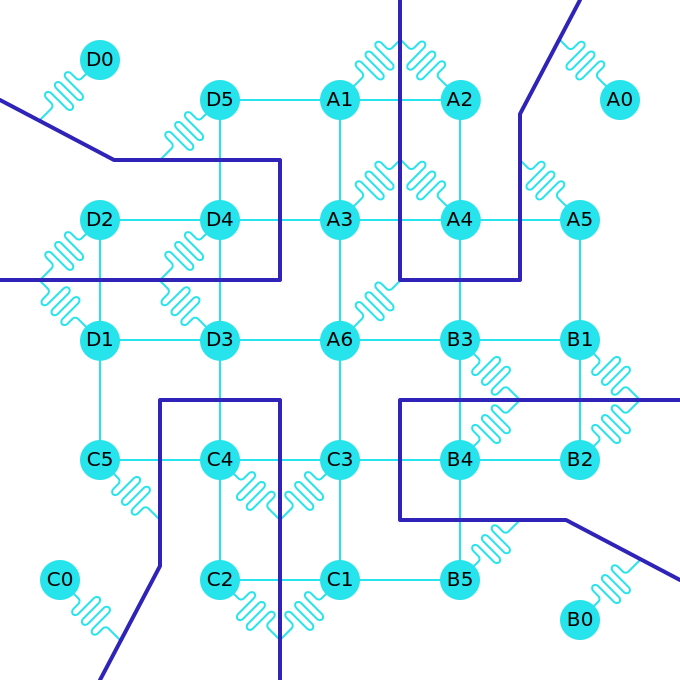
\includegraphics[width=0.80\textwidth]{figures/png/qw11q.jpeg}
        \subcaption{}
        \label{fig:qw11q_picture}
    \end{subfigure}
    \hfill
    \begin{subfigure}{0.50\textwidth}
        \centering
        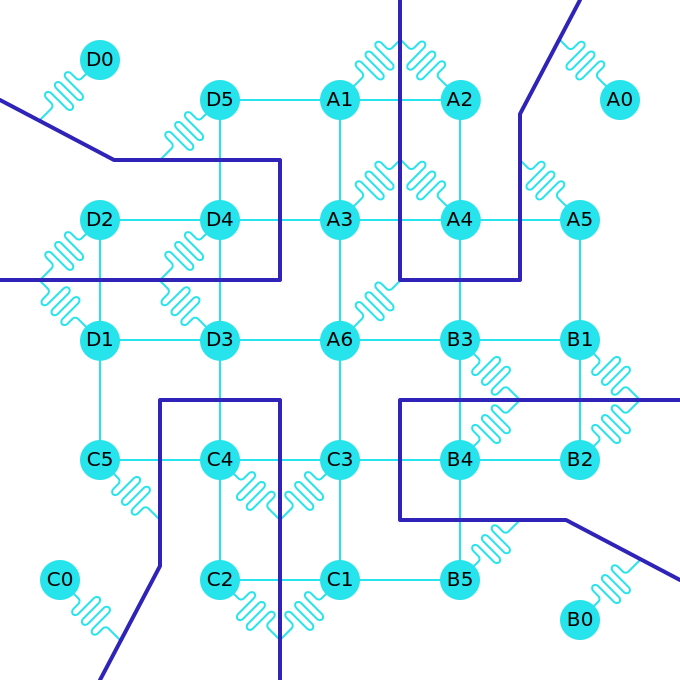
\includegraphics[width=\textwidth]{figures/png/qw11q.png}
        \subcaption{}
        \label{fig:qw11q_topology}
    \end{subfigure}
    \caption{Figure \ref{fig:qw11q_picture}: Picture of the Contralto-D chip from QuantWare. Figure \ref{fig:qw11q_topology}: Topology of the Contralto-D chip from QuantWare.}
    \label{fig:qw11q}
\end{figure}

As discussed in the previous chapter, the behavior of Josephson junctions and SQUIDs relies critically on the superconducting state of the materials involved. 
To achieve and maintain this regime, it is essential that the superconducting elements operate well below their critical temperature. 
For this reason, the Contralto-D chip is installed at the lowest temperature stage of the cryostat, where the required thermal conditions for superconductivity are met. 
This ensures the proper functioning of the quantum hardware and enables the realization of coherent quantum operations.

These systems achieve ultra-low temperatures by exploiting the unique quantum properties of helium-3 (\ce{^{3}He}) and helium-4 (\ce{^{4}He}) isotopes in a dilution process.
At the core of a dilution refrigerator is a mixing chamber, where the cooling mechanism takes place. 
When a mixture of \ce{^{3}He} and \ce{^{4}He} is cooled below approximately 870 millikelvin, the two isotopes phase-separate into a \ce{^{3}He}-rich phase and a \ce{^{3}He}-dilute phase. 
The key principle is that when \ce{^{3}He} atoms cross the phase boundary—from the concentrated phase into the dilute phase—they absorb energy from their surroundings. 
This process is endothermic and is the fundamental source of cooling in the dilution refrigerator.\\
The system operates as a closed loop: \ce{^{3}He} gas is circulated using a combination of sorption pumps and still pumps, which remove \ce{^{3}He} vapor from the still (typically at $600–800$ mK), recondense it at a higher stage, and reintroduce it into the mixing chamber. 
The refrigerator includes several thermalization stages—typically at $50$ K, $4$ K, $800$ mK, $100$ mK, and finally below $20$ mK—each connected to a corresponding cooling stage and separated by radiation shields and thermal filters to minimize heat load and noise from higher-temperature stages.
Dilution refrigerators are highly stable and capable of reaching base temperatures below $10$ mK, with hold times on the order of days or even weeks. 
These temperatures are crucial for achieving the low thermal noise and long coherence times necessary for high-fidelity quantum operations in superconducting circuits.
Specifically the cryostat employed in the lab is the XLDsl from Bluefors \cite{XLD1000}, an image of the cryostat is shown in Figure \ref{fig:XLDsl}.

\begin{figure}[h!]
    \centering
    \includegraphics[width=0.35\textwidth]{figures/png/XLD1000.png}
    \caption{Picture of the XLDsl dilution refrigerator at the QRC Lab}
    \label{fig:XLDsl}
\end{figure}

Outside the cryostat, the control and readout of superconducting qubits are managed by dedicated room-temperature electronics.
These systems are responsible for generating the microwave pulses used to drive single- and two-qubit gates, as well as for acquiring and processing the output signals that encode the qubit states 
Typically they include arbitrary waveform generators (AWGs), microwave sources, mixers, digitizers, and field-programmable gate arrays (FPGAs).
The generated microwave pulses are shaped and modulated at room temperature before being attenuated and routed to the cryogenic environment. 
Similarly, signals returning from the qubits are amplified and digitized for state discrimination and further processing. 
The electronics employed in the lab for the control of the \tt{qw11q} is the OPX1000 platform by Quantum Machines \cite{opx1000}.

The software I used for the calibration of the qubits and the subsequent experiments is \Qibocal (\cite{pasquale_qibocal_2024}, \cite{qibocalscience}, \cite{qibocalgit}), while the backend for communication with the laboratory instruments is \Qibolab (\cite{efthymiou_qibolab_2024}, \cite{qibolabscience}, \cite{qibolabgit}).
\Qibolab is the control layer responsible for managing and executing low-level instructions on the hardware, bridging high-level quantum models and physical quantum platforms.
It is designed to support diverse experimental setups and allows the researcher to define custom hardware configurations through a platform abstraction and to execute custom pulse sequences using both commercial and open-source firmware.
The communication between \Qibolab and the quantum hardware is structured and modular, relying on a stack that includes instrument drivers, pulse control logic, and a compiler that translates abstract quantum gates into hardware-specific instructions.
This structure enables compatibility with heterogeneous platforms and facilitates the development of experimental drivers tailored to different laboratory environments.
\Qibocal interfaces directly with \Qibolab to apply calibration protocols on the physical device. The routines deployment takes place through the interpretation of declarative runcards written in YAML.
\Qibocal allows an easy execution of pulse sequences, collection of measurement data, and interpretation of the results through the reports that are automatically generated upon completion of the routine.

\section{Single qubit calibration experiments}

The first task that I needed to complete at the beginning of my thesis work was the calibration of at least a line of the superconducting quibts of the Contralto-D chip using the \Qibocal library.
From this point onward, for the sake of brevity, I will refer to the chip interchangeably as Contralto-D or \tt{qw11q}, which is the name of the node under which it is registered on the QRC computing cluster.
In the following I will describe the experiments that I performed and commenting on the results.

\subsection{Resonator calibration}
Before starting with the calibration of the gates necessary for quantum computing it is necessary to charachterize the qubit an clibrate the readout pulses. 
For this reason the calibration process starts with the charachterization of the resonator coupled to the qubit that will be used to perform non-destructive measurements of the qubit state.

\subsubsection{Resonator spectroscopy}
The first step to calibrate the readout pulse is to charachterize the resonator is to find the resoinator frequency, that is the tranisition frequency for the resonator. 
At this frequency, a distinct difference in the transmitted signal can be observed depending on the type of resonator used. 
In the case of a 3D cavity resonator, the signal appears amplified, whereas for a 2D planar resonator, the signal tends to be more strongly absorbed. Regardless of the resonator type, the response typically exhibits a Lorentzian-shaped peak: this peak is positive for 3D cavities due to the amplification effect, and negative for 2D resonators due to their greater absorption.

The outcome of this experiment is strongly influenced by the amplitude of the excitation pulse. 
To reliably determine the resonator frequency, the pulse duration can be fixed on the order of microseconds, which is sufficient to observe the relevant signal response.
However, selecting an appropriate amplitude requires more careful consideration. When the amplitude is high, the signal becomes more prominent, improving the signal-to-noise ratio (SNR) and making it easier to identify the resonator's response.
If the amplitude is increased too much, however, it can drive the system out of the superconducting regime.  
In this case, the resonator becomes effectively decoupled from the qubit, and the frequency observed corresponds to the so-called bare resonator frequency.
During the first calibration operations it is not necessary to have the qubit coupled to the resonator but is helpful to improve the SNR to have a more defined peak in the signal, for this reason the first calibration routines are run in a high-power regime.

In this experiment the main variables on which the experimenterer can operate are the frequency range that is willing to scan and the step of the scan. 
Regarding the frequency range a very wide scan can be useful if nothing is known about the studied resonator, but usually the design parameters are provided by the produttore; t is possible that they are not exact, but can give an idea of the region to scan.
Regarding the step for the scan, usually a step of 200 MHz can be used to probe the resonator frequency but can be reduced if a more precise scan is needed. 
An example of measurement of the bare resonator frequency is shown in Figure \ref{fig:res_high}.
 
\begin{figure}[h!]
    \centering
    \includegraphics[width=\textwidth]{figures/png/res_spectroscopy_high.png}
    \caption{Output of resonator spectroscopy with high power on qubit B2.}
    \label{fig:res_high}
\end{figure}

An example of the measurement of the resonator frequency in the low-power regime is shown in Figure \ref{fig:res_low}.

\begin{figure}[h!]
    \centering
    \includegraphics[width=\textwidth]{figures/png/res_low.png}
    \caption{Output of resonator spectroscopy with low power on qubit B2.}
    \label{fig:res_low}
\end{figure}

Uno studio più preciso della risposta del risonatore può essere realizzato eseguendo la routine di resonator spectroscopy cambiando la funzione di fit,  questa variazione dell'esperimento è descritta nell'appendice \hyperref[app:AppendixA]{Appendix A}

\subsubsection{Resonator punchout}
After having found the bare resonator frequency it is necessary to identify the resonator frequency under qubit coupling. 
To do this it is possible to repeat the spectroscopy, this time over a narrower frequency range and for varying pulse amplitudes. 
The resonator frequency is expected to depend strongly on amplitude: it remains constant in the high-power regime, shifts during an intermediate transition phase, and stabilizes again at a different value once the qubit-resonator interaction becomes significant.
For this calibration protocol the experimenterer must carefully choose the frequency and amplitude range to scan to avoid extremly long experiments, at the same time the frequency and amplitude steps must be small enough to clearly identify the frequency and amplitude in which the shift happens.   

%The expected result from a resonator punchout experiment is shown in Figure \ref{fig:res_punchout}
%\begin{figure}[h!]
%    \centering
%    \includegraphics[width=\textwidth]{figures/png/res_punchout.png}
%    \caption{Output of resonator punchout on qubit B2.}
%    \label{fig:res_punchout}
%\end{figure}

\subsubsection{Resonator flux dependence}
As explained in section \ref{subsec:flux_tunable_transmon} it is suggested to work at the qubit sweetspot, where the qubit frequency is less sensitive to magnetic flux fluctuations.
For this reason, it is useful to estimate the location of the sweet spot prior to performing qubit spectroscopy, enabling measurements to be carried out near the optimal bias point. 
This can be accomplished by exploiting the qubit–resonator coupling: since the qubit frequency depends on the magnetic flux, as shown in equation \ref{eq:freqdepndenceonflux}, and the qubit is coupled to the resonator, the resonator frequency also exhibits a flux dependence. 
The resonator detuning in the transmon regime ($E_J \gg E_C$) can be computed as 
\begin{equation}\label{eq:resonator_flux_dependence}
    f_r(\Phi) = f_r^{\text{bare}} + \frac{g^2 \sqrt[4]{d^2 + (1 - d^2) \cos^2 \left( \pi \frac{\Phi}{\Phi_0} \right)}}{f_r^{\text{bare}} - f_q(\Phi)},
\end{equation}
where $f_r^{\text{bare}}$ is the bare resonator frequency, $g^2$ is the coupling between the transmon and the resonator, $d$ is the junctions asymmetry, $E_C$ is the charging energy, $E_J$ the Josephson energy and $\Phi_0 = h/2e$ is the flux quanta.

In \Qibocal it is possible to perform a resonator flux dependence experiment to measure and fit and the curve described by Eq. \ref{eq:resonator_flux_dependence}.
With this routine the experimenter performs a scan of the both the external bias and frequency, thihs experiment provides an approximate indication of the sweetspot.
An example of the output of this experiment is shown in Figure

%\begin{figure}[h!]
%    \centering
%    \includegraphics[width=\textwidth]{figures/png/res_punchout.png}
%    \caption{Output of resonator punchout on qubit B2.}
%    \label{fig:res_punchout}
%\end{figure}

\subsection{Qubit calibration}
After having determined all the readout parameters it is possibile to continue the calibration process by calibrating the qubit.

\subsubsection{Qubit spectroscopy}
To determine the resonance frequency of a qubit, a qubit spectroscopy experiment is performed, which, unlike resonator spectroscopy, requires a two-tone approach. 
While resonator spectroscopy is typically a single-tone measurement used to identify the resonator's response, qubit spectroscopy involves applying a drive tone to the qubit followed by a readout tone to detect the qubit state. 
This method becomes essential after an initial estimate of the readout frequency and amplitude has been obtained from a resonator punchout experiment. 
In this protocol, a drive pulse of variable frequency $\omega$ is sent through the qubit drive line. 
If the drive frequency is far detuned from the qubit transition frequency $\omega_{q}$, it will have no appreciable effect on the qubit state, and the measured signal will remain unchanged. 
However, as $\omega$ approaches $\omega_{01}$ the drive pulse can induce transitions between the qubit states. 
This excitation modifies the qubit population and, consequently, the resonator response, which is sensitive to the qubit state due to their dispersive coupling. 
When the drive frequency is near resonance and the pulse is sufficiently long, the qubit may reach a maximally mixed state leading to a detectable change in the readout signal amplitude. 
By sweeping the drive frequency and recording the corresponding readout amplitudes, one can plot a spectroscopy curve that reveals a Lorentzian dip or peak centered at the qubit transition frequency—opposite in direction to the Lorentzian feature observed in the resonator spectroscopy, due to the nature of the state-dependent dispersive shift.

An example of the output of qubit spectroscopy experiment is shown in Figure \ref{fig:qubit_spectroscopy}
\begin{figure}[h!]
    \centering
    \includegraphics[width=\textwidth]{figures/png/qubit_spectroscopy.png}
    \caption{Output of qubit spectroscopy on qubit B2.}
    \label{fig:qubit_spectroscopy}
\end{figure}

\subsubsection{Qubit EF spectroscopy}
Qubit spectroscopy can also be extended to probe transitions to higher excited states beyond the first excited state. 
Directly observing these higher-level transitions typically requires significantly increased drive power, which may exceed the safe operational limits of the experimental setup. 
An alternative and more controlled approach involves first preparing the qubit in state $\ket{1}$, followed by a standard spectroscopy sequence to induce the $\ket{1} \leftrightarrow \bra{2}$ transition. 

%\begin{figure}[h!]
%    \centering
%    \includegraphics[width=\textwidth]{figures/png/ef.png}
%    \caption{Output of qubit spectroscopy to identify the transition frequency between state $\ket{1}$ ($\ket{e}$) and state $\ket{f}$ (first scited state) on qubit B2.}
%    \label{fig:ef}
%\end{figure}

Note that the description of this calibration routine has been included here for the sake of clarity and continuity of exposition; however, since it requires the qubit to be in the $\ket{1}$ state at the beginning of the spectroscopy, it can only be performed after the execution of a single-shot classification (see Section \ref{subsec:single_shot}).

\subsubsection{Qubit flux dependence}
By performing a resonator flux dependence the experimenterer obtained a first estimate for the sweetspot, now by performing a qubit flux spectroscopy.
In this experiment a constant DC current signal is sent to the qubit through the flux line with voltage and amplitude fixed for the bias level and then a qubit spectroscopy is performed.
This procedure is repeated  for different bias levels and different drive frequencies.
The expected result of the routine is shown in Figure \ref{fig:qubit_flux}.

When calibrating the qubit sweetspot it is important to consider that on a superconducting qubatum chip qubits are not completely isolated systems; rather, they interact with one another through both intentional couplings (e.g capacitive or inductive couplers) and unintended cross-talk mechanisms. 
The mutual influence that qubits exert on each other's affect their effective operating parameters, particularly their flux-dependent transition frequencies.
This means that also the location of the sweetspot can be affected by the biasing of neighboring qubits, this occurs because the flux-tuning circuitry is not perfectly isolated; biasing one qubit can induce a spurious flux in nearby qubits, effectively shifting their frequency spectra and hence their sweetspots.
Consequently, calibrating each qubit in isolation may yield misleading results, therefore, to accurately determine and operate all qubits at their true sweetspots under realistic experimental conditions, it is important to perform simultaneous calibration. 
This ensures that all mutual interactions and cross-couplings are properly accounted for, leading to a more stable and predictable multi-qubit operation.

\begin{figure}[h!]
    \centering
    \includegraphics[width=\textwidth]{figures/png/qubit_flux.png}
    \caption{Output of the qubit flux dependence on qubit B2.}
    \label{fig:qubit_flux}
\end{figure}

\subsubsection{Qubit crosstalk}
To perform a more detailed study of the qubit crosstalk it is possible to perform a \tt{qubit\_crosstalk} experiment.

\subsection{Drive pulse calibration}

After defining all the readout parameters and the parameters for qubit control, it is necessary to calibrate the parameters of the drive pulses to be able to control rotations on the Bloch sphere.
With Rabi experiments is possibile to calibrate the drive pulses to perform precise rotations (see \cite{Rabi1936}, \cite{Wallraff2005}) within approximately $40$ ns.
This duration is typical for single-qubit gates in superconducting qubit systems, as it represents a balance between fast control and minimal spectral leakage. 
Faster gates would require higher drive amplitudes, which can increase errors due to leakage into higher transmon levels or induce unwanted transitions in nearby qubits through cross-resonance or crosstalk effects \cite{TransmonPaper}, \cite{Motzoi_2009}. 
On the other hand, significantly longer gates are more susceptible to decoherence, particularly due to $T_1$ relaxation and $T_2$ dephasing processes, which limit overall gate fidelity \cite{Barends2014-pb}.

Usually the first step of calibrating drive pulses consists in calibrating a $\pi$-pulse, namely an $X$-gate. 
The goal of the Rabi experiment is to tune the amplitude or duration of the drive pulse, in order to excite the qubit from the ground state up to state $\ket{1}$.

\subsubsection{Rabi oscillation experiments}
To experimentally probe the coherent control of a qubit in \Qibocal it is possible to perform different variations of the Rabi oscillation experiments, which provides direct evidence of the qubit's ability to undergo controlled rotations under a resonant microwave drive, as described in Section \ref{sec:qubit_control}.
In this experiment, a microwave pulse of the form  

\begin{equation}\label{eq:microwave_pulse}
    V_d(t) = A \varepsilon(t) \sin(\omega_d t + \alpha),
\end{equation}
is applied through the control line (XY line), and coupled capacitively to the qubit. 
The qubit is initialized in its ground state $\ket{0}$, and the drive frequency $\omega_d$ is set close to the qubit transition frequency $\omega_q$. 
The envelope $\varepsilon(t)$ is typically Gaussian, and its shape is kept constant throughout the experiment. 
The key parameter that is varied is the amplitude $A$ of the drive pulse (or alternatively, the duration of the pulse while keeping amplitude constant).

To better understand the evolution of the system, it is possible to consider the driven qubit in the interaction picture. 
The qubit state can be written as:
\begin{equation}\label{eq:general_state}
    \ket{\psi(t)} = C_0(t) e^{+i \omega_q t/2} \ket{0} + C_1(t) e^{-i \omega_q t/2} \ket{1}.
\end{equation}
%
Solving the time-dependent Schr\"odinger equation for state \ref{eq:general_state} under Hamiltonian\ref{eq:interaction_hamiltonian} yields the following expressions:
\begin{align}
    C_0(t) &= e^{-i \Delta_d t / 2} \left[ \cos \left( \frac{\Omega_R t}{2} \right) + i \frac{\Delta_d}{\Omega_R} \sin \left( \frac{\Omega_R t}{2} \right) \right], \\
    C_1(t) &= i \frac{\Omega}{\Omega_R} e^{i \Delta_d t / 2} \sin \left( \frac{\Omega_R t}{2} \right),
\end{align}
where $\Delta_d = \omega_q - \omega_d$ is the detuning, and
\begin{equation}
    \Omega_R = \sqrt{\Omega^2 + \Delta_d^2},
\end{equation}
is the generalized Rabi frequency.

The probability of finding the qubit in the excited state at time $t$ is given by:
\begin{equation}
    P_1(t) = |C_1(t)|^2 = \frac{\Omega^2}{\Omega^2 + \Delta_d^2} \sin^2 \left( \frac{\Omega_R t}{2} \right).
\end{equation}
This result shows that the probability oscillates in time with frequency $\Omega_R$, and the amplitude of the oscillation is reduced when the drive is off-resonant ($\Delta_d \neq 0$).
The closer the drive is to resonance, the higher the probability of full excitation.

In the resonant case, when $\omega_d =\omega_q$ and $\Delta_d = 0$ the generalized Rabi frequencyreduces to $\Omega_R = \Omega$ and the excited state probability becomes
\begin{equation}\label{eq:rabi_amplitude}
    P_e (t) = P_1(t) = \sin^2\left(\frac{\Omega t}{2} \right) = \frac{1}{2}(1-\cos(\Omega t)),
\end{equation}
which is the curve that is used in the fit when performing a Rabi amplitude experiment.

An example of the output of a Rabi amplitude experiment is shown in figure \ref{fig:rabi_amplitude}.
\begin{figure}[h!]
    \centering
    \includegraphics[width=\textwidth]{figures/png/rabi_amp.png}
    \caption{Output of the Rabi amplitude routine on qubit B2.}
    \label{fig:rabi_amplitude}
\end{figure}

A variation of the Rabi amplitude experiment consists of the Rabi length experiment, where instead of the amplitude, the parameter that is varied is the duration of the drive pulse.
The qubit is again initialized in the ground state $\ket{0}$ and subjected to a resonant microwave drive ($\omega_d = \omega_q$). 
In this case, the pulse envelope $\varepsilon(t)$ and amplitude $A$ are held constant, while the total duration of the pulse is incrementally varied. 
This enables the observation of coherent oscillations in the excited state population as a function of pulse length. 
However, unlike the idealized scenario, in realistic conditions the qubit experiences energy relaxation and dephasing, which attenuate the oscillation amplitude over time. 
To account for these effects, the excited state probability is modeled as represents the effective decay time, incorporating both energy relaxation and dephasing processes.
\begin{equation}
    P_e (t) = P_1(t)= \frac{1}{2}\left(1- e^{-t/\tau}\cos(\Omega_R \frac{t}{2})\right),
\end{equation}
where $\Omega_R$ is the generalized Rabi frequency and $\tau$ 

\begin{figure}[h!]
    \centering
    \includegraphics[width=\textwidth]{figures/png/rabi_length.png}
    \caption{Output of the Rabi length routine on qubit B2.}
    \label{fig:rabi_length}
\end{figure}


Sometimes, when the qubit frequency is not precisely known, or when systematic effects such as pulse distortions, frequency drifts, or cross-talk may affect the calibration it can be useful to perform a Rabi measurement in which the amplitude and frequency of the drive pulse are scanned.
In \Qibocal this experiment is implemented as the Rabi amplitude-frequency routine, this experiment provides a comprehensive view of the qubit's response to a range of drive conditions and is particularly useful during initial calibration.
This experiment reveals a characteristic chevron-shaped interference pattern in the excitation probability as a function of drive frequency and amplitude. 
Figure \ref{fig:rabi_amplitude_frequency} shows a possible output of this experiment, in the plot in figure in particular it is possible to see only the first region of the chevron shape with high probability of finding the qubit in an excited state.

\begin{figure}[h!]
    \centering
    \includegraphics[width=\textwidth]{figures/png/rabi_af.png}
    \caption{Output of the Rabi amplitude-frequency routine on qubit B2.}
    \label{fig:rabi_amplitude_frequency}
\end{figure}

\subsection{Fine-tuning calibration}

\subsubsection{Ramsey experiment}\label{subsec:Ramsey}
After calibrating the readout and $\pi$-pulses, technically should be possible to execute algorithmic experiments on the qubit. 
However, essential characteristics of the qubit, such as its coherence properties and the precise drive frequency, remain to be determined; without this information, circuit fidelities would be suboptimal. 
The Ramsey experiment is a simple yet powerful protocol that allows simultaneous investigation of multiple aspects of qubit behavior, including the fine tuning of the drive frequency and verification of coherent control and signal phase consistency. 
It also enables extraction of the qubit's coherence time $T_2^*$.

In its standard implementation, the Ramsey sequence consists of two $\frac{\pi}{2}$-pulses separated by a variable delay $\tau$.\\
The first $\frac{\pi}{2}$-pulse brings the qubit from the ground state $\ket{0}$ onto the equatorial plane of the Bloch sphere, placing it in a superposition of $\ket{0}$ and $\ket{1}$.
During the delay $\tau$, he qubit state accumulates a relative phase due to its Larmor precession and environmental noise, effectively evolving around the z-axis.\\
The second $\frac{\pi}{2}$-pulse projects the final state back onto the measurement basis, and the probability of measuring the excited state $\ket{1}$ is recorded.
Repeating this procedure for different delay times $\tau$ allows to monitor the decay of coherence in the qubit state.

In the ideal, non-detuned case, where the drive frequency matches the qubit transition frequency, the observed signal exhibits a purely exponential decay toward a baseline value, from which the characteristic decoherence time $T_2^*$ can be extracted.
However, small deviations from the ideal $\frac{\pi}{2}$-pulse, due to imperfect calibration or a mismatch between the drive and quibt frequency lead to more complex behaviour.

Usually a small intentional detuning is applied, in this case the measurement outcomes show a sinusoidal modulation superimoposed on the exponential decay so that the reuslting curve can be fitted with the equation \cite{Baur2012RealizingQG}
\begin{equation}\label{eq:Ramsey}
    p_e(\tau) = \frac{1}{2} + \frac{1}{2}e^{-\tau/T_2^*}\cos{(\Delta\omega \tau)},
\end{equation}
An example of the output of a Ramsey experiment is shown in Figure \ref{fig:ramsey}

\begin{figure}[h!]
    \centering
    \includegraphics[width=\textwidth]{figures/png/ramsey.png}
    \caption{Output of the Ramsey amplitude routine on qubit B2.}
    \label{fig:ramsey}
\end{figure}

\subsubsection{Flipping experiment}

While the Ramsey experiment is typically used to fine-tune the drive frequency of a qubit, the Flipping experiment serves as an effective routine to calibrate the amplitude of the $\pi$-pulse, ensuring accurate implementation of $R_x(\pi)$ rotations. 
This calibration is fundamental for achieving high-fidelity gate operations, and the flipping experiment can often reveal discrepancies in the amplitude that are not evident in Rabi oscillation measurements.\\
In this protocol, a flip is defined as a pair of consecutive $\pi$-pulses, which ideally return the qubit to its initial state due to a full $2\pi$ rotation. 
The experiment begins with the qubit initialized in the ground state $\ket{0}$, followed by an $R_x(\pi/2)$ rotation that places it in an equal superposition state on the equator of the Bloch sphere. 
Without the initial $R_x(\pi/2)$ rotation, errors in the $\pi$-pulses would lead only to a global phase difference, which is not detectable via projective measurements. 
With the superposition state, however, the qubit's evolution becomes sensitive to amplitude miscalibrations, allowing over- and under-rotations to be distinguished through changes in measurement probability.

Following the initial $\pi/2$-pulse, the qubit is subjected to a number $N$ of flips choosen by the experimenter. 
After the flips, a projective measurement is performed. This procedure is repeated for increasing values of $N$, effectively building a scan of how the qubit state evolves under repeated application of imperfect $\pi$-pulses.

In the ideal case, where the $\pi$-pulse amplitude is perfectly calibrated, the repeated flips return the qubit to the equatorial plane after each cycle, resulting in a constant measurement probability. 
The recorded signal should appear as a flat line; however, if the amplitude is miscalibrated, the qubit state will drift on the Bloch sphere, leading to oscillatory behavior in the measured population as a function of the number of flips. 
This deviation is modeled by a sinusoidal function, from which the amplitude error can be quantitatively extracted.
Figure \ref{fig:flipping} shows the result of a flipping routine.

\begin{figure}[h!]
    \centering
    \includegraphics[width=\textwidth]{figures/png/flipping.png}
    \caption{Output of the flipping routine on qubit B2.}
    \label{fig:flipping}
\end{figure}

\subsubsection{Dispersive shift}
A possible strategy to improve the assignment fidelity is to perform a dispersive shift measurement which helps calibrate the readout frequency.
To calibrate the readout frequency based on the dispersive shift, two resonator spectroscopy measurements are performed. 
In the first, the resonator response is measured while the qubit remains in its ground state $\ket{0}$, effectively treating the system as a bare resonator. 
In the second measurement, a calibrated $\pi$-pulse is applied before each acquisition to prepare the qubit in the excited state $\ket{1}$, and the spectroscopy is repeated under otherwise identical conditions. 
The transmission or reflection spectra from both configurations are then plotted together as a function of probe frequency. 
At each frequency point, single-shot measurements are collected, and the resulting IQ data are analyzed. 
Specifically, the distance between the centroids of the two resulting IQ distributions, one corresponding to the ground state and the other to the excited state, is computed. 
The readout frequency that maximizes this centroid separation is selected, as it provides the greatest distinguishability between the two qubit states and thus optimizes the readout contrast.

A typical result for this routine is shown in Figure \ref{fig:dispersive_shift}

\begin{figure}[h!]
    \centering
    \includegraphics[width=\textwidth]{figures/png/dispersive_shift.png}
    \caption{Output of the Rabi amplitude routine on qubit B2.}
    \label{fig:dispersive_shift}
\end{figure}

\subsection{Qubit charachterization}
\subsubsection{T1 \& T2 measurement}
After having calibrated all the parameters concerning the qubit it is possible to proceed with charachterization experiments such as $T1$ and $T2$ measurements.

As explained in Section \ref{subsec:qubit_decoherence}, due to coupling to the environment the qubit in state $\ket{1}$ will decay to the state $\ket{0}$. 
To measure the charachteristic decay time $T_1$ it is possible to perform a simple experiment where the qubit is initialized in state $\ket{1}$ using a previously calibrated $\pi$ pulse.
After a variable delay $\Delta\tau$, during which the qubit undergoes spontaneous decay due to coupling to the environment, a projective measurement is performed.
For $\Delta\tau = 0$ we expect to fin the qubit in state $\ket{1}$ while for $\Delta\tau \rightarrow \infty$ the system relaxes fully to the ground state $\ket{0}$.
r intermediate times, the probability of finding the qubit in $\ket{1}$ decays exponentially, and the measured excited state population $p_e(t)$ as a function of time $t$ is fitted to the model 
\begin{equation}\label{eq:T1}
    p_e(t) = A + Be^{-\frac{t}{T_1}},
\end{equation}
where $T_1$ is the exnergy relation time and $A$, $B$ are the fitting parameters.
The expected result from this routine is shown in Figure \ref{fig:t1}.

\begin{figure}[h!]
    \centering
    \includegraphics[width=\textwidth]{figures/png/t1.png}
    \caption{Output of the $T1$ measurement on qubit B2.}
    \label{fig:t1}
\end{figure}

After measuring $T_1$ it is necessary to measure also the dephasing time of the qubit, $T_2$; to do this in \Qibocal, it is possible to perform a T2 experiment.
The acquisition sequence of the experiment is the same as the Ramsey experiment described in Section \ref{subsec:Ramsey}: a pair of $\pi/2$-pulses is applied with a variable delay $\tau$ in between, during which the qubit freely evolves under a slightly detuned drive.
As a result, the measured excited state population exhibits oscillations in time, caused by the accumulation of phase due to the detuning. 
These oscillations are enveloped by an exponential decay that reflects the qubit’s loss of phase coherence over time.  

In the T2 experiment the same pulse sequence is used with the caveat that the drive pulse is not detuned, the protocol assumest that any error on the drive frequency has already been corrected through a Ramsey experiment.
For this reason the curve that describes the excited state population is expected to follow a simple exponential decay:
\begin{equation}
    p_e(t) = A + Be^{-\frac{t}{T_2}},
\end{equation}
where $A$ and $B$ are two fitting parameters.

\begin{figure}[h!]
    \centering
    \includegraphics[width=\textwidth]{figures/png/t2.png}
    \caption{Output of the $T2$ measurement on qubit B2.}
    \label{fig:t2}
\end{figure}

\subsubsection{Single shot classification}\label{subsec:single_shot}
At this stage of the calibration procedure, the drive and measurement pulses have been individually calibrated, while a measurement now yields a clear analog output, this alone does not indicate whether the qubit was in state $\ket{0}$ or $\ket{1}$.
To establish this correspondence and enable digital state assignment, it is necessary to perform a single-shot readout experiment.

To charachterize the readout configuration of a superconducting qubit, the measurement is performed using a heterodyne detection setup (see \cite{gao_practical_2021}, \cite{krantz_quantum_2019}) which acquires the transmitted microwave signal from the readout resonator.
Although the average signal clearly distinguishes the two states, in a single instance, often called single shot, th signal is noisy. 
This noise arises both from quantum fluctuations intrinsic to the electromagnetic field inside the resonator and from added noise contributed by amplifiers and other electronics in the detection chain.
The raw signal, sampled over a finite window, is digitally integrated to produce a single complex number corresponding to one measurement instance.
Repeating this process after preparing the qubit in a known state produces a cloud of points in the complex IQ plane \cite{krantz_quantum_2019}.
For both state $\ket{0}$ and state $\ket{1}$ we typically observe one Gaussian-shaped distribution of IQ values The separation between these two clusters originates from the dispersive interaction between the qubit and the resonator, which induces a state-dependent frequency shift and consequently a distinguishable phase shift in the transmitted microwave tone. 
Since the acquisition integrates the signal over time, each shot produces a single point whose location reflects the qubit state but is blurred by noise that generates the Gaussian distributions.

The readout calibration experiment starts by preparing the qubit in state $\ket{0}$, letting it relax to its ground state and collecting IQ data without averaging.
The experiment is then repeated the after applying a $\pi$-pulse to prepare the qubit in state $\ket{1}$ and the unavaraged IQ-values are recorded.
Plotting all these single shots in the IQ plane reveals two roughly circular clusters. 

To classify the measured IQ points, the centroids of the two Gaussian-like distributions corresponding to the qubit prepared in $\ket{0}$ and $\ket{1}$ are first identified. 
The axis passing through these centroids is used to define the direction along which the state information is most distinguishable. 
The IQ plane is then rotated so that this axis aligns with the horizontal (real) axis, concentrating the relevant state-dependent variation along a single dimension. 
This rotation is characterized by an angle, measured in radians, between the centroid-connecting axis and the original $Q$-axis.

Following the rotation, the coordinate system is translated such that the centroid of the ground state distribution is placed at the origin. 
All IQ points are then projected onto the real axis, and the resulting one-dimensional distributions for each state are analyzed. 
The cumulative distribution functions of these projections are computed, and the optimal threshold is determined by finding the point that maximizes the absolute difference between the two distributions. 
This threshold defines the decision boundary used to assign a binary qubit state to any new measurement, based on its projection along the rotated axis.

The quality of the classification is then quantified by the assignment fidelity, defined as \cite{gao_practical_2021} 
\begin{equation}
    \mathcal{F} = \ -\frac{1}{2}(P(0,1)+P(1,0)),
\end{equation}
where $P(i,j)$ is the probability of measuring the qubit in state $i$ but prepared in state $j$; this fidelity is typically expected to exceed 90–95\% for a well-calibrated readout. 
It serves as a crucial figure of merit for the qubit, reflecting how reliably one can distinguish its quantum states in a single-shot measurement. 

The result of the classification routine should be similar to the one showed in Figure \ref{fig:classification}.

\begin{figure}[h!]
    \centering
    \includegraphics[width=0.4\textwidth]{figures/png/classification.png}
    \caption{Output of the single shot classification on qubit B2.}
    \label{fig:classification}
\end{figure}


\subsection{Standard Randomized Benchmarking}
The standard randomized benchmarking experiment will be described in more detail in the following chapter (see Section \ref{sec:RBsection}).
For now it is enough to say that in this routine, sequences of randomly selected Clifford gates are applied to the qubit, followed by an inverting gate that ideally returns the system to its initial state. 
By measuring the survival probability as a function of sequence length and fitting the decay curve, an estimate of the average gate fidelity is obtained.
An example of the output expected from the randomized benchmarking protocol is shown in Figure \ref{fig:rb}.

\begin{figure}[h!]
    \centering
    \includegraphics[width=0.85\textwidth]{figures/png/rb.png}
    \caption{Output of the standard randomized benchmarking routine on qubit B2.}
    \label{fig:rb}
\end{figure}


\subsection{DRAG experiment}\label{sec:DRAG}
\subsubsection{DRAG pulse shape}
As mentioned in section \ref{sec:qubit_control}, the study of optimal pulse shapes (especially for drive and control pulses) is an active area of research. 
The Derivative Reduction by Adiabatic Gate (DRAG) technique \cite{Motzoi_2009}\cite{Gambetta_2011} is a widely used method to mitigate leakage errors during high-fidelity single-qubit gate operations.
The DRAG is the analytical solution to force the interaction Hamiltonian of the system \ref{eq:interaction_hamiltonian} to be restricted to the computational space.

The DRAG scheme implements a single-qubit rotation by applying a shaped pulse with an envelope $\Omega(t)$ on one quadrature (typically along $\hat{\sigma_x}$) and a secondary pulse with an envelope proportional to the time derivative $\dot{\Omega}(t)$ on the orthogonal quadrature (typically $\hat{\sigma_y}$).
For instance, a rotation about the $x$-axis is generated by the time-dependent Hamiltonian\cite{manenti_quantum_2023}:
\begin{equation}\label{eq:DRAG_hamiiltonian}
    \hat{H}_d(t) = \hbar \, \Omega_x(t) \sin(\omega_d t) \, \hat{\sigma}_x + \hbar \, \Omega_y(t) \sin(\omega_d t + 2\pi) \, \hat{\sigma}_y,
\end{equation}
where the pulse shapes are defined as:
\begin{align}
    \Omega_x(t) &= \Omega_0 e^{-t^2 / (2\sigma^2)}, \\
    \Omega_y(t) &= \lambda_\eta \frac{d}{dt} \Omega_x(t),
\end{align}
where $\eta$ represents the qubit anharmonicity and $\lambda$ is a dimensionless scaling parameter.
The efficacy of the DRAG correction arises from its ability to suppress virtual transitions that occur due to the spectral overlap of the primary pulse with off-resonant transitions in the multilevel qubit structure.

Theory predicts that setting $\lambda=1$ minimizes the leakage to higher excited stats, while $\lambda=0.5$ is optimal for correcting phase distortions induced during the gates \cite{Motzoi_2009}, \cite{Gambetta_2011}, \cite{Motzoi2013}.
In experimental implementations, the optimal value of $\lambda$ may deviate from theoretical predictions due to pulse distortions, limited bandwidth of the control electronics, and interactions with the readout resonator \cite{PhysRevA.82.040305}.

\subsubsection{DRAG protocol}
A straightforward experiment implemented in \Qibocal to calibrate the $\lambda$ parameter involves performing two separates measurments using DRAG pulses in the pulse sequence.
In the first experiment, a sequence of DRAG pulses is applied in the order $Y_{\pi}$$X_{\frac{\pi}{2}}$ with both pulses parametrized by a given value of $\lambda$. 
For the second measurement the procedure is the same but the pulse order is reversed $X_{\pi}$$Y_{\frac{\pi}{2}}$.
These specific sequences are chosen because they ideally result in the same final quantum state—any discrepancy between the two indicates phase misalignment, in particular these sequences exhibit opposite signs of phase errors, as explained in \cite{reed2013entanglementquantumerrorcorrection}. 

The post-processing consist in measuring the probability of the qubit being in the state $\ket{1}$ for each value of $\lambda$. 
A linear fit is performed for both pulse sequences, and the correct $\lambda$ is the value where the two lines cross. 
This intersection corresponds to the $\lambda$ value that minimizes phase errors and ensures the qubit operates with minimal distortion.

An example of the expected output for the DRAG routine is shown in Figure \ref{fig:drag}
\begin{figure}[h!]
    \centering
    \includegraphics[width=0.65\textwidth]{figures/png/drag_simple.png}
    \caption{Expected output of the DRAG routine. $\beta$ is the symbol used in \Qibocal for the $\lambda$ parameter.}
    \label{fig:drag}
\end{figure}

\section{Calibration results}

In Table \ref{tab:cal_results}, are summarized the results obtained for the calibration of line D of the \tt{qw11q} chip. 
The readout and assignment fidelities were obtained by performing a classification exèperiment on each qubit with 5000 shots, while $T1$ and $T2$ measurements were carried out using the respective protocols, each with $2048$ shots.\\
The standard randomized benchmarking was performed at four different circuit depths: $n=1,5,10,20$; for each depth the circuit was repeated $20$ times with $100$ shots per repetition. 
The number of shots in the randomized benchmarking experiment was deliberately limited, as this routine is inherently very time-consuming.

\begin{table}[h]
    \centering
    \begin{tabular}{lccccc}
    \toprule
    \textbf{Qubit} & \textbf{Readout Fidelity} & \textbf{Assignment Fidelity} & \textbf{T1 [$\mu$s]} & \textbf{T2 [$\mu$s]} & \textbf{Gate infidelity (e-3)} \\
    \midrule
    \textbf{D1} & $0.876$ & $0.938$ & $26.4 \pm 0.4$ & $13.0 \pm 2.0$ & $27.0 \pm 21.0$ \\
    \textbf{D2} & $0.945$ & $0.973$ & $14.9 \pm 0.1$ & $18.0 \pm 10.0$ & $20.5 \pm 6.2$ \\
    \textbf{D3} & $0.905$ & $0.952$ & $23.6 \pm 0.3$ & $28.0 \pm 12.0$ & $7.0 \pm 18$ \\
    \textbf{D4} & $0.929$ & $0.964$ & $20.6 \pm 0.2$ & $40.0 \pm 5.2$ & $4.4 \pm 4.8$ \\
    \bottomrule
    \end{tabular}
    \caption{Single qubit gates calibration results.}
    \label{tab:cal_results}
\end{table}

The values of the assignment fidelity and readout fidelity are overall satisfactory, indicating reliable state discrimination during measurement. 
Similarly, the relaxation time $T_1$ of the qubit shows acceptable values.

On the other hand, the coherence time $T_2$ is generally low, especially when considering that its theoretical upper bound is $2T_1$. 
This indicates the presence of significant pure dephasing mechanisms, which are limiting the coherence independently of energy relaxation processes. 
A reduced $T_2$ can have important consequences for subsequent experiments, particularly impacting the performance of randomized benchmarking protocols. 
Specifically, a short coherence time may degrade the fidelity of gate operations, leading to an overestimation of the average error per gate. 

%%%results
\chapter{RB fidelity optimization}
The calibration procedure described in Section \ref{sec:calibration} is typically time-consuming and demands significant experimental expertise, particularly when aiming for state-of-the-art performance. 
In the work I presented in the previous chapter, the calibration process began from a pre-existing, even if suboptimal, configuration. 
The goal was to enhance the quality of single-qubit gates by using the available \Qibocal protocols.

Even under these ovverall favorable initial conditions, the effort required to refine gate performance showed the limitations of manual calibration approaches. 
As quantum processors scale in both qubit count and architectural complexity, manual calibration becomes increasingly complex. 
Frequent recalibrations are necessary to mitigate the effects of parameter drift and environmental fluctuations, especially in superconducting qubit platforms \cite{krantz_quantum_2019}.

Furthermore, as gate fidelities approach the fault-tolerance threshold, enabling practical quantum computation across a variety of applications, accurate control of single-qubit gates becomes essential. 
The fidelity of an individual gate quantifies its average operational performance, directly impacting circuit-level error rates and representing a critical figure of merit for quantum processors. 
However, improving gate fidelity remains challenging because of the nontrivial mapping between gate parameters and the underlying process matrix, and errors from state preparation and measurement (SPAM) can make it difficult to distinguish between different sources of error.

In this chapter, i present an initial attempt to address the dual challenges of calibration complexity and residual gate errors. 
The goal is to find calibration procedures that are not only effective but also repeatable and accessible to non-expert users, lowering the entry barrier for experimental optimization of superconducting qubits. 
Building on the approach proposed in \cite{kelly_optimal_2014}, which demonstrated that optimizing the sequence fidelity at a fixed length of randomized benchmarking (RB) can improve gate performance, we explored an automatic recalibration procedure based on randomized benchmarking fidelity as an optimization target.

The focus of this first study is the optimization of single-qubit gate fidelity, that was chosen both for its foundational importance and its relative accessibility compared to more complex operations.
Starting from single-qubit gates thus provides a practical and effective testbed for validating optimization algorithms before extending them to more complex multi-qubit operations.
The results presented in this chapter shows how different optimization strategies perform when applied to improving gate fidelity in realistic experimental settings.

\section{Randomized Benchmarking}\label{sec:RBsection}
A strong limitation to the realization of quantum computing technologies is the loss of coherence that happens as a consequence of the application of many sequential quantum gates to to the quibts.
A possible approach to characterize gate error is the quantum process tomography which allows the experimenter to establish the behaviour of a quantum gates. 
The main drawback of this approach is that process tomography can be very time consumig since its time complexity scales exponentially with the number of qubits involved \cite{QPTomography} and the result is affected by state preparation and measurements (SPAM) errors.

To overcome these limitations, randomized benchmarking (RB) was introduced and is currently widely used to quantify the avarage error rate for a set of quantum gates.

The main idea is that the error resulting from the combined action of random unitary gates, which are drawn from a uniform distribution according to the Haar measure \cite{Mele_2024} and applied sequentially to the qubit, averages out to effectively behave like a depolarizing channel \cite{Emerson_2005_RB}.
This last consideration simplifies the characterization of noise because it removes dependence on specific error structures and allows fidelity to be extracted through a simple exponential decay.

It was later shown that it is possible to simplify this procedure even more, by restricting the unitaries to gates in the Clifford group \footnote{unitary rotations mapping the group of Puali operators in itself} and by not requiring that the sequence is strictly self-inverting \cite{knill_randomized_2008}.
The fundamental principle of RB is the application of sequences of randomly selected quantum gates from the Clifford group $\mathcal{C}$ followed by an inversion gate which, in absence of noise, return the system to its initial state. 
For real systems, where noise is present, the observed survival probability provides an estimate of the avarage gate fidelity.

The standard RB protocols consist of the following steps:\begin{enumerate}\label{routine:RB}
    \item Initialize the system in ground state $\ket{0}$
    \item For each sequence-length $m$ build a sequence of $m$ randomly drawn Clifford gates $C_1, C_2, ..., C_m$
    \item Determine the inverse gate $C_{m+1}=(C_m\circ...\circ C_1)^{-1}$
    \item Measure $C_{m+1}\circ C_m \circ ...\circ C_1 \ket{0}$
\end{enumerate}
The process must be repeated for multiple sequence of the same length and with varying length.

In an ideal systems, without noise, we should have 
\begin{equation}\label{eq:CliffordIdeal}
    C_{m+1}\circ C_m \circ ...\circ C_1 \ket{0} = (C_m\circ...\circ C_1)^{-1}\circ(C_m\circ...\circ C_1)\ket{0} = \ket{0}.
\end{equation}
However in real systems Equation \ref{eq:CliffordIdeal} does not hold; instead randomization with Clifford gates behave as a depolarizing channel \ref{eq:depolarizing_channel} with depolarization probability $d$.\\
The survival probability of the initial state $\ket{0}$ for different sequence lengths $m$ follows the exponential decay model \begin{equation}\label{eq:RB_decay}
    F(m) = Ap^m +B,
\end{equation}
where $1-p$ is the rate of depolarization and $A$ and $B$ capture the state preparation and measurement errors.\\
The parameter $p$ is directly related to the depolarization probability $d$ through the avarage gate fidelity $F$ which, for a depolarizing channel, is given by \begin{equation}
    F = 1 - \frac{d}{2^n - 1}\label{eq:avarage_gate_fidelity},
\end{equation}
where $n$ is the nuber of qubits.
%For the details of the calculations to obtain eq. \ref{eq:avarage_gate_fidelity} see \hyperref[app:AppendixC]{Appendix C}.
The avarage error per Clifford gate $\varepsilon_{Clifford}$ can be computed as \begin{equation}
    \varepsilon_{Clifford} = 1 - F \label{eq:avg_error_Clifford_gate},
\end{equation}
where $F$ is the avarage gate fidelity. 
Sobstituting in \ref{eq:avg_error_Clifford_gate} the formula for the avarage gate fidelity \ref{eq:avarage_gate_fidelity} we obtain \begin{equation}
    \varepsilon_{Clifford} = \frac{d}{2^n -1} = \frac{1-p}{1-2^{-n}},
\end{equation}
which shows how the avarage error per Clifford gate is directly connected to the exponential decay rate.

\section{RB evaluation and optimization}
%TODO: inserire una introduzione per questa sezione

\subsection{\Qibolab native gates}
As discussed at the beginning of the chapter, the primary goal of this work is to explore an automated calibration approach aimed at optimizing the single-gate fidelity of logical gates. 
In particular, we focused on the calibration of the $R_X$ gate, which corresponds to a microwave pulse with a specific frequency, amplitude, and duration that induces a rotation of the qubit state by an angle of $\pi$ around the $x$-axis of the Bloch sphere.

The choice to optimize the $R_X$ gate dependes on its role as one of the native gates in the \texttt{Qibolab} control stack. 
Native gates are physical operations that are directly implementable by the hardware, in contrast to abstract logical gates, which must be compiled into sequences of these hardware-supported primitives. 
In the case of \texttt{Qibolab}\footnote{At least for version 0.1 of \Qibolab}, the native gate set consists of $R_X$ pulses combined with virtual-Z (VZ) gates. 
This native gate basis is both efficient to implement and expressive enough to support universal quantum computation.

Indeed, it can be shown that any arbitrary single-qubit unitary operation $ U(\gamma, \theta, \phi) \in SU(2) $ can be expressed, up to a global phase, as a sequence of rotations around the $z$ and $x$ axes of the Bloch sphere:
\begin{equation}
U(\gamma, \theta, \phi) = R_Z(\gamma) R_X(\theta) R_Z(\phi).
\end{equation}
This decomposition ensures that all single-qubit operations can be realized using a combination of $ R_X $ and $ R_Z $ rotations. 

When a qubit is driven by a resonant microwave pulse (with detuning $ \delta = 0 $), the resulting evolution is a rotation around an axis $\hat{n} = (\cos\phi, -\sin\phi, 0)$ lying in the equatorial plane of the Bloch sphere. 
The associated unitary can be written as:
\begin{equation}
R_{\hat{n}(\phi)}(\theta) = \exp\left( -i \frac{\theta}{2} \left[ \cos(\phi)\sigma_x - \sin(\phi)\sigma_y \right] \right).
\end{equation}

This operation can be equivalently expressed through conjugation of an $R_X$ rotation by two $R_Z$ rotations:
\begin{equation}
R_{\hat{n}(\phi)}(\theta) = R_Z(-\phi) R_X(\theta) R_Z(\phi) = U(-\phi, \theta, \phi).
\end{equation}
From this, it follows that any arbitrary unitary $ U(\gamma, \theta, \phi) $ can be implemented as:
\begin{equation}
U(\gamma, \theta, \phi) = R_Z(\gamma + \phi) \cdot R_Z(-\phi) R_X(\theta) R_Z(\phi) = R_Z(\gamma + \phi) \cdot U(-\phi, \theta, \phi).
\end{equation}

Note that, in practice, this final $R_Z$ rotation does not need to be realized as a physical pulse. 
Instead, it can be implemented virtually by adjusting the phase reference of subsequent pulses, a technique known as the virtual-Z gate\cite{McKay_2017}. \\
The ability to compose any single-qubit gate using only $R_X$ and virtual-Z operations \cite{boykin1999universalfaulttolerantquantumcomputing} confirms the sufficiency of this native gate set for universal single-qubit control. For instance, even a restricted $ R_X $ rotation such as $ R_X(\pi) $, when combined with arbitrary-angle $ R_Z $ gates, forms a universal set due to the non-commuting nature of these operations. By alternating $ R_X(\pi) $ pulses with phase-adjustable $ R_Z $ gates, one can synthesize any $ SU(2) $ unitary up to global phase.

Given these consideration, the optimization experiments described in the following sections focus on maximizing the $R_X$ gate fidelity using RB fidelity as a performance metric. 

\subsection{RB evaluation parameters}
In the results presented in the following, I employed the randomized benchmarking (RB) routine implemented in \Qibocal, an example of which is shown in Section \ref{sec:RB_calibration}. 
This routine was used consistently across all tests, with the following set of parameters: I used $1000$ unique random Clifford sequences (\texttt{num\_of\_sequences = 1000}), ensuring robust statistical reliability across different realizations of gate noise. 
Each sequence was evaluated at increasing circuit depths up to a maximum of $1000$ Clifford gates (\texttt{max\_circuit\_depth = 1000}), with the depths spaced by increments of $10$ (\texttt{delta\_clifford = 10}), resulting in benchmarking points at depths of $1, 10, 20, \ldots, 1000$. 
For each depth and random sequence, I generated only one instance (\texttt{n\_avg = 1}), meaning that each sequence was distinct and not repeated with the same gate pattern. 
Consequently, statistical averaging was achieved across the ensemble of random sequences at each depth rather than by repeating individual circuits. 
To ensure high confidence in the estimation of the survival probabilities, each circuit was executed with $2000$ measurement shots. %TODO: verify and check
\footnote{All experiments and results presented in this chapter were performed using version 0.1 of \Qibocal. This means that the parameters used to execute the \texttt{rb\_ondevice} routine, as described above, refer specifically to version 0.1. At the time of writing, version 0.2 of \Qibocal has been released and is actively maintained. As a result, the available parameters for running the RB routine may have changed and might no longer correspond exactly to those described in this text.}

\subsection{Parametri da ottimizzare}
%TODO: descrivere quali parametri sto cercando di ottimizzare, per quali gate, perchè quella gate (è la mia native gate) e come procedo (quindi prima cerco di fare un fine tuning)
%descrivere anche il fatto che in realtà questo procedimento di fine tuning non è così banale e che può decisamente influenzare i risultati (spiegare come sono inizializzati i parametri per l'ottimizzazione)
I parametri su cui è stata performata l'ottimizzazione sulla base della gate infidelity ottenuta dall'RB come cost function sono 3 (voglio ottimizare la porta logica $RX(\pi)$): frequenza, ampiezza e forma dell'impulso.
Per quanto rigaurda la forma dell'impulso in particolare il parametro da ottimizzare era il parametro $\beta$ dell'impulso di DRAG, vale a dire il parametro moltiplicativo sulla seconda quadratura.
Questo significa che la closed loop optimization che è stata realizzata è avvenuta secondo un procedimento simile a quello descritto nel paper ORBIT \cite{kelly_optimal_2014}
%TODO: spiegare un attimo meglio che cos'è ORBIT (Optimal Randomized Benchmarking)

%TODO: inserire code snippet dove mostro come inizializzo i parametri 


In un secondo momento invece è stata valuata anche l'evoluzione della gate fidelity ottenuta tramite RB ottimizzando solamente i parametri di ampiezza e frequenza dell'$RX(\pi)$ e tenendo un impulso Gaussiano.


%TODO: try to run at least once the NM from not-fine tuned

\section{Scipy optimization methods}\label{Sec:OptimizationMethods}

\subsection{Algorithm description}
The initial optimization attempts were carried out using standard algorithms available in the \texttt{SciPy} library \cite{SciPy-NMeth}.
In the following sections, I present the specific algorithm used and discuss the results obtained from its application to the problem of gate fidelity optimization.

\subsubsection{Nelder-Mead}
The first gradient-free optimization method to be tested was Nelder-Mead since in letteratura era già stato riportato il suo utilizzo per obiettivi simili \cite{kelly_optimal_2014}.

The Nelder-Mead optimization method, originally introduced by Nelder and Mead in 1965 \cite{NelderMeads}, is a widely used numerical optimization technique for unconstrained problems in multidimensional spaces. \\
This derivative-free method is operates using simplex, which is a polytope of $n+1$ vertices in a $n$-dimensional space.
The algorithm iteratively updates the simplex by replacing its worst-performing vertex with a new candidate point, thereby guiding the search towards an optimal solution. 
If the goal is to minimize a given function $f(\mathbf{x})$ where $\mathbf{x} \in \mathbb{R}^n$ the algorithms proceeds with the following steps:\begin{enumerate}
    \item If not otherwise initialized, $n+1$ points are sampled for building the initial symplex
    \item \tt{Order} the test points according to their values at vertices: $f(\mathbf{x}_1) \leq f(\mathbf{x}_2) \leq \dots \leq f(\mathbf{x}_{n+1})$ and check whether the algorithm should terminate.
    \item \tt{Calculate} $\mathbf{x}_0$, the centroid of all points except $\mathbf{x}_{n+1}$.
    \item \tt{Reflection}: Compute the reflected point $\mathbf{x}_r = \mathbf{x}_0 + \alpha(\mathbf{x}_0 - \mathbf{x}_{n+1})$ with $\alpha > 0$. 
            If $\mathbf{x}_r$ satisfies $f(\mathbf{x}_1) \leq f(\mathbf{x}_r) < f(\mathbf{x}_n)$, then a new simplex is obtained by replacing the worst-performing point $\mathbf{x}_{n+1}$ with $\mathbf{x}_r$ and then go to step 1.
    \item \tt{Expansion}: If $\mathbf{x_r}$ is the current best point, meaning that $f(\mathbf{x}_r) < f(\mathbf{x}_1)$, then the expanded point is computed: $\mathbf{x}_e = \mathbf{x}_0 + \gamma(\mathbf{x}_r-\mathbf{x}_0)$ with $\gamma>1$.
           If $\mathbf{x}_e$ satisfies $f(\mathbf{x}_e) < f(\mathbf{x}_r)$, then a new simplex is obtained by replacing $\mathbf{x}_{n+1}$ with the expanded point $\mathbf{x}_e$ and then go to step 1.\\
            If instead $f(\mathbf{x}_e) \geq f(\mathbf{x}_r)$, the new simplex is obtained by replacing $\mathbf{x}_{n+1}$ with $\mathbf{x}_r$, and then go to step 1.
    \item \tt{Contraction}: In this case is certain that $f(\mathbf{x}_r) \geq f(\mathbf{x}_n)$ then:\begin{itemize}
        \item If $f(\mathbf{x}_r) < f(\mathbf{x}_{n+1})$: compute the contracted point $\mathbf{x}_c=\mathbf{x}_0 +\rho(\mathbf{x}_{r}-\mathbf{x}_0)$ with $0<\rho \leq 0.5$.
                If $\mathbf{x}_c$ satisfies $f(\mathbf{x}_c) < f(\mathbf{x}_{r})$, then a new simplex is obtained by replacing $\mathbf{x}_{n+1}$ with  $\mathbf{x}_c$ and go to step 1.\\
                Else go to step 6.
        \item  If $f(\mathbf{x}_r) \geq f(\mathbf{x}_{n+1})$: compute the contracted point $\mathbf{x}_c=\mathbf{x}_0 +\rho(\mathbf{x}_{n+1}-\mathbf{x}_0)$ with $0<\rho \leq 0.5$.
                If $\mathbf{x}_c$ satisfies $f(\mathbf{x}_c) < f(\mathbf{x}_{n+1})$, the a new simplex is constructed with $\mathbf{x}_c$ and go to step 1.\\
                Else go to step 6.
    \end{itemize}
    \item \tt{Shrinkage}: Replace all points except the best, $\mathbf{x}_1$, with $\mathbf{x}_i = \sigma(\mathbf{x}_i - \mathbf{x}_1), 0<\sigma \leq 0.5$  
\end{enumerate}
The algorithm terminates when the standard deviation of the function values of the current simplex fall below a user-initialized tolerance. 
When the cycle stops the point of the simplex associated to the lower function value is returned as proposed optimum

The values of the parameters $\alpha, \gamma, \rho$ and $\sigma$ were left to default of \tt{scipy}: $\alpha=1, \gamma=2, \rho=0.5, \sigma=0.5$. 

\subsubsection{SLSQP}
Per valutare eventuali miglioramenti nella performance abbiamo provato ad utilizzare un algoritmo che fosse gradient-based. 
Nello specifico ho provato ad utilizzare l'algoritmo di Sequential Least Squares Programming (SLSQP) nella versione implementata all'interno della libreria scipy.
Method SLSQP uses Sequential Least SQuares Programming to minimize a function of several variables with any combination of bounds, equality and inequality constraints. 
The method wraps the SLSQP Optimization subroutine originally implemented by Dieter Kraft \cite{kraft1988slsqp}.  
Note that the wrapper handles infinite values in bounds by converting them into large floating values.

Sequential Least Squares Programming (SLSQP) is a numerical algorithm designed for solving constrained nonlinear optimization problems of the general form:
\begin{align*}
& \min_{x \in \mathbb{R}^n} \quad && f(x) \\
& \text{subject to} \quad && c_i(x) = 0, \quad i = 1, \dots, m \\
& && d_j(x) \geq 0, \quad j = 1, \dots, p
\end{align*}

It belongs to the family of Sequential Quadratic Programming (SQP) methods, which iteratively solve a sequence of quadratic programming subproblems that approximate the original nonlinear problem. 
At each iteration, the nonlinear objective function is replaced by a quadratic model, and the constraints are linearized around the current iterate. 
The resulting subproblem is a quadratic program whose solution provides a direction for updating the optimization variables.

The quadratic model is typically derived from the Lagrangian function associated with the problem,
\begin{equation}
\mathcal{L}(x, \lambda, \mu) = f(x) - \sum_{i} \lambda_i c_i(x) - \sum_{j} \mu_j d_j(x),
\end{equation}
where $ \lambda $ and $ \mu $ are the Lagrange multipliers associated with the equality and inequality constraints, respectively. 
The Hessian of the Lagrangian is not computed explicitly; instead, SLSQP employs a quasi-Newton approximation, updated using a BFGS-like scheme. 
Although it does not implement the BFGS algorithm in the strict sense, the use of such updates places SLSQP within the broader class of quasi-Newton SQP algorithms.

A constrained line search is performed along the computed search direction to ensure sufficient decrease in a merit function that balances objective reduction and constraint satisfaction. 
This ensures both global convergence and rapid local convergence near a solution. 
The process continues until convergence criteria, typically based on the projected gradient norm and constraint residuals, are satisfied.

\subsection{Results}
In the following I present the results obtained provando ad effettuare l'ottimizzaione con l'algoritmo di Nelder-Meads

\begin{tabular}{lcccccc}
    \textbf{Method} & \textbf{Success} & \textbf{Status} & \textbf{Objective Value} & \textbf{Iterations} & \textbf{Duration}\\
    \textbf{Nelder-Mead} & False & 2 & 0.002732 & 40 & 93 & No initial symplex\\
    \textbf{Nelder-Mead}
\end{tabular}

\section{CMA-ES}

\subsection{Algorithm description}
Covariance Matrix Adaptation Evolution Strategy (\tt{CMA-ES} \cite{cmaessimplepractical}), is a population-based evolutionary algorithm designed for optimizing complex, non-convex, and high-dimensional functions.\\
It belongs to the broader class of Evolution Strategies (ES), a subset of Evolutionary Algorithms (EAs)(see \cite{sloss20192019evolutionaryalgorithmsreview}), and is particularly effective for black-box optimization where gradient information is unavailable.

Evolution Strategies (ES) are a class of optimization methods that employ self-adaptive mechanisms to explore the search space efficiently. 
Unlike classical optimization techniques that rely on gradient descent, ES leverage stochastic sampling to navigate rugged and multimodal landscapes.
In this context, CMA-ES is an adaptive stochastic search method that iteratively refines a probability distribution over the search space. 
Unlike traditional Genetic Algorithms (GAs), which rely on crossover and mutation operators, CMA-ES employs a multivariate normal distribution to generate candidate solutions. 
The method adaptively updates the distribution's mean and covariance matrix based on the fitness of sampled points.

The fundamental idea behind CMA-ES is the use of a multivariate Gaussian distribution to model promising search directions. 
Let $\mathbf{\mu}_t$ denote the mean of the distribution at iteration $t$, and $\Sigma_t$ the covariance matrix. 
Then, a new population of $\lambda$ candidate solutions $\mathbf{x}_i^(t+1) \sim \mathbf{\mu}_t + \sigma_t\mathcal{N}(0, \Sigma_t)$, where $\sigma_t$ is a step size controlling the exploration.  

The CMA-ES algorithm follows the following steps:\begin{enumerate}
    \item If not otherwise specified, the initial parameters are set: mean vector $\mathbf{\mu_0}$, covariance matrix $\Sigma_0$\footnote{$\Sigma_0=\mathbb{I}$ for isotropic search}, step size $\sigma_0$, population size $\lambda$
    \item Generate $\lambda$ new candidate solutions $\mathbf{x}_i$ according to a multivariate normal distribution.
    \item Evaluate the objective function $f(\mathbf{x}_i)$ for each candidate solution.
    \item Sort the new candidate solutions based on fitness: $f(\mathbf{x}_0) \leq ... \leq f(\mathbf{x}_{\lambda})$.
    \item Update the mean vector $\mathbf{\mu}$ with the $m=\lfloor \lambda / 2 \rfloor$ top performing solutions:\begin{equation}
        \mathbf{\mu} \leftarrow \sum_{i=0}^m \mathbf{w}_i\mathbf{x}_1,
    \end{equation} where $\mathbf{w}_i$ are internally defined weights.
    \item Update the isotropic and anisotropic evolution path $\mathbf{p}_{\sigma}$, $\mathbf{p}_c$ \footnote{For details on the update process of the evolution paths see \cite{cmaessimplepractical}.}.
    \item Update the covariance matrix: \begin{equation}
        C \leftarrow (1 - c_1 - c_{\mu}) C + c_1 \mathbf{p}_c \mathbf{p}_c^T + c_{\mu} \sum_{i=1}^{\mu} w_i \mathbf{y}_i \mathbf{y}_i^T,
    \end{equation} where $c_1$ and $c_\mu$ are learning rates and $\mathbf{y}_i$ represents the deviation of the $i$-th cnadidate solution from the mean $\mathbf{mu}$.
    \item Update the step size using a cumulative path evolution mechanism \begin{equation}
        \sigma \leftarrow \sigma \cdot \exp \left( \frac{c_{\sigma}}{d_{\sigma}} \left( \| \mathbf{p}_{\sigma} \| - E \| \mathcal{N}(0, I) \| \right) \right),
    \end{equation} where $c_\sigma$ is the learning rate for step-size adaptation, $d_\sigma$ is a damping factor $\| \mathbf{p}_{\sigma} \|$ is the length of the evolution path and $E \| \mathcal{N}(0, I) \|$ is the expected length of a standard normally distributed random vector.
\end{enumerate}

Nel seguito, a meno che non sia diversamente specificato, i parametri sono stati inizializzati ai valori di default della libereria \tt{CMA-ES}
\subsection{Results}


\section{Optuna}

\subsection{Algorithm description}

In addition to the optimization methods mentioned earlier, the Tree-Structured Parzen Estimator (TPE) method was employed, using its implementation available in the \texttt{optuna} library \cite{optuna_2019}.

Tree-Structured Parzen Estimator (TPE) is a Sequential Model-Based Optimization (SMBO) approach \cite{SMBO_proceedings}. 
SMBO methods sequentially construct models to approximate the performance of optimization parameters based on historical measurements, and then subsequently choose new parameters values to test based on this model. \cite{BayesianOptimizationReview}
At the heart of SMBO is the idea of building a surrogate model, which is used to predict the objective function's values for unseen parameters configurations. 
The surrogate model is iteratively updated as new observations are made, and the optimization process balances exploration, which focuses on uncertain regions of the search space, and exploitation, which focuses on areas that are more likely to improve the objective based on past evaluations. 
This balance ensures that the optimization process makes efficient use of resources and avoids wasting time on suboptimal regions.\\

The TPE algorithm is a probabilistic model-based optimization method that uses non-parametric density estimation to guide the search. 
The TPE algorithm differs from traditional Bayesian optimization approaches, such as Gaussian Process-based methods, in its modeling strategy. 
Rather than directly approximating the objective function, TPE constructs two separate probabilistic models:

\begin{itemize}
    \item $p(x | y < y^*)$, the likelihood of observing a parameter configuration $x$ given that the objective function value $y$ is below a chosen threshold $y^*$.
    \item $p(x | y \geq y^*)$, the likelihood of observing $X$ for less promising function values.
\end{itemize}

These probability densities are estimated using non-parametric methods such as kernel density estimation (KDE). 
New candidate points are then generated by sampling from $p(x | y < y^*)$, favoring configurations that are expected to yield lower objective values. The threshold $y^*$ is typically set as a quantile of observed values, ensuring a focus on the most promising regions of the search space.

The TPE method is the default optimization strategy in \tt{Optuna}, an advantage in the optimization algorithm as implemented in optuna is the addition of an authomatic \textit{pruning} mechanism that stops  unpromising trials early, which can significantly speed up the optimization process by avoiding unnecessary computations.
In our case, this is particularly relevant because the execution of the RB routine, which is performed at each call to the cost function, requires [insert approximate execution time]

As implemented in our code, the default pruner used is the median pruner \tt{optuna.pruners.MedianPruner}. 
This pruner works by evaluating the intermediate results of a trial and comparing them to the median of completed trials at the same step. 
If the current trial's performance is worse than the median, it is pruned to prevent wasting computational resources on unpromising configurations. 

\subsection{Results}

\subsection{$\beta$ parameter impact on RB optimization}

\paragraph{D1 - steps}

\paragraph{D1 - 1000 steps}

\paragraph{D2 - 1000 steps}



\section{RB optimization conclusions}

\begin{tabular}{lccccc}
    \textbf{Method} & \textbf{Highest Fidelity} & \textbf{Amplitude [a.u.]} & \textbf{Frequency [GHz]} & \textbf{$\beta$} \\

\end{tabular}
\chapter{Pulses analysis and tuning}
\section{RX90 calibration}
Another possible source of error is ...

\section{Flux pulse correction}
\subsection{Notes on signal analysis}


\subsection{Cryoscope}
The experiment that we describe in this section was first introduced in \cite{rol_time-domain_2020}, the goal is to determine predistortions that needs to be applied to a flux pulse signal so that the qubit receives the flux pulse as intended by the experimenter.

As explained in section \ref{sec:cQED}, accurate dynamical control of qubit frequency is of key importance to realize single- and two-qubit gates.
One of the on-chip control variable that is used on QunatumWare chip is the magnteic flux through a SQUID loop, the signal for magnetic flux control originates from an arbitrary waveform genarator (AWG) which operates at room temperature.\\
As the signal propagates through various electrical components along the control line leading to the quantum device it undergoes linear dynamical distortions. 
If not properly compensated, these distortions can degrade gate performance, impacting experiments fidelity and repeatability.\\

In \cite{rol_time-domain_2020} is proposed a technique to characterize flux-pulse distortions induced by components inside the dilution refrigerator by directly measuring the qubit state.
In this protocol we send the qubit a pulse sequence where a flux pulse of varying duration $\tau$ is embedded between two $\frac{\pi}{2}$ pulses which are always separated by a fixed interval $T_{sep}$.\\
The first $\frac{\pi}{2}$ pulse rotates the qubit of $\frac{\pi}{2}$ around the $y$ axis of the Bloch sphere changing its state from $\ket{0}$ to $\frac{\ket{0}+\ket{1}}{\sqrt{2}}$.
If no flux pulse was applied, during $T_{sep}$ the qubit would decohere around the $z$ axis, leaving the qubit in state $\ket{\psi(T_{sep})} = \exp \left\{-i\frac{\omega_Q T_{sep}}{2}\hat{\sigma}_z\right\}$ where $\omega_Q$ is the qubit frequence.\\

When a flux pulse $\Phi_{Q,\tau}(t)$ of duration $\tau$ is sent to the qubit\footnote{To send a $\Phi_{Q,\tau}(t)$ flux pulse we are actually sending a $V_{\text{in},\tau}(t)$ voltage pulse through the electronics} after the first $\frac{\pi}{2}$ pulse, the qubits evolve to the state $\frac{\ket{0}+e^{i\varphi_\tau}\ket{1}}{\sqrt{2}}$ with relative quantum phase 
\begin{equation}\label{eq:phi}
    \frac{\varphi_{\tau}}{2\pi} = \int_{0}^{T_{sep}} \Delta f_Q (\Phi_{Q,\tau(t)})\text{d}t = \int_{0}^{\tau} \Delta f_Q (\Phi_{Q,\tau(t)})\text{d}t + \int_{\tau}^{T_{sep}} \Delta f_Q (\Phi_{Q,\tau(t)})\text{d}t
\end{equation}
where in the second step I separate the contributions from flux response up to $\tau$ and the turn-off transient. For a full derivation of equation eq. \ref{eq:phi} see \hyperref[app:AppendixB]{Appendix B}.
\subsubsection{Pulse reconstruction}

\subsubsection{Corrections study}

\subsection{Corrected pulse}

\begin{comment}
    TO DO LIST:
    * calcoli analitici per assunzioni del cryoscope
    * calcoli analitici di convoluzioni per dimostrare che è giusto il modo in cui combiniamo i filtri
    * costruire script per analisi dati
    * eventualmente provare ad aggiungere più correzioni esponenziali
\end{comment}
\subsection{Filter determination}
\subsubsection{IIR}
\subsubsection{FIR}
for description and notes on \tt{CMA-ES} see section \ref{Sec:OptimizationMethods}
\subsubsection{Output filters in QM}


\chapter{Conclusions}
%\input{Conlusions}

\backmatter
%BIBLIOGRAPHY
\printbibliography
\chapter*{Appendix A} 
\addcontentsline{toc}{chapter}{Appendix A}
\markboth{Appendix A}{Appendix A}
\label{app:AppendixA}

A more accurate description of the resonance profile for a two-dimensional notch-type resonator is provided in the literature \cite{Gao2008}, where the transmitted signal is modeled as a complex function of frequency. 
The complete expression for the complex transmission coefficient is given by

\begin{equation}
S_{21}(f) = ae^{i\alpha}e^{-2\pi i f \tau}\left[ 1 - \frac{(Q_l/|Q_c|)e^{i\phi}}{1 + 2iQ_l(f/f_r -1)} \right].
\end{equation}

This formulation provides a deeper insight into both the environmental and resonator-specific contributions to the observed response. 
The prefactor accounts for the attenuation and gain in the measurement chain through the amplitude $a$, introduces a global phase shift $\alpha$, and models the effect of finite cable length via a frequency-dependent delay term characterized by the parameter $\tau$. 
These components collectively represent systematic effects that shape the baseline response of the system.

The second part of the expression captures the physical behavior of the resonator itself. 
It includes the loaded quality factor $Q_l$, which reflects the total energy loss in the system, and the coupling quality factor $Q_c$, which quantifies the interaction between the resonator and the transmission line. 
The resonance frequency $f_r$ marks the center of the frequency response, while the phase offset $\phi$ accounts for impedance mismatches and Fano-type interferences caused by reflections within the setup.
This model exploits all the information encoded in both the magnitude and phase of the complex transmission signal, allowing for a more comprehensive characterization. 

\paragraph{}
However, directly fitting the complete model involves a nonlinear optimization over seven parameters, which is inherently sensitive to initial conditions and often non-robust. 
To improve the stability and reliability of the fitting process, the problem is decomposed and approached in stages, each targeting a subset of parameters.

First, the cable delay is estimated by fitting a linear function to the phase response across frequency. 
The delay introduces a phase tilt proportional to the frequency, and its removal reveals the underlying circular shape of the resonance response in the complex plane. 
Once the delay is corrected, a geometric circle fit is performed on the data.

Then the phase angle $\theta$ is fit according to the following expression:
\begin{equation}
    \theta(f) = \theta_0 - 2\pi \tau (f - f_r) + 2 \arctan \left[ 2 Q_l \left( 1 - \frac{f}{f_r} \right) \right],
\end{equation}
where an additional linear term accounts for any residual cable delay not captured in the initial correction. 
This protocol is implemented in \Qibocal and available by selecting the \tt{s21} fitting routine for the resonator spectroscopy, an example of the expected output obtained from running such experiment is shown in Figure \ref{fig:res_s21}.

\begin{figure}[ht!]
    \centering
    \includegraphics[width=\textwidth]{figures/png/s21.png}
    \caption{Output of resonator spectroscopy performed with \tt{s21} fit function.}
    \label{fig:res_s21}
\end{figure}

\chapter*{Appendix B}
\addcontentsline{toc}{chapter}{Appendix B}
\markboth{Appendix B}{Appendix B}
\label{app:AppendixB}

In general, it is possible to show that for different forms of the detuning flux 
\begin{equation}\label{eq:det_flux}
    \Delta f(\Phi) = a\Phi^k
\end{equation}
where $k \in \mathbb{Z}^+$, the relative phase $\varphi_{\tau}$ can be calculated as follows:
\begin{align}
    \varphi_\tau &= 2\pi a \int_{0}^{\infty} \left[ \int_{0}^{\infty} h(t - t') dt' - \int_{0}^{\infty} h(t - \tau - t') dt' \right]^k dt \\
    &= 2\pi a \int_{0}^{\tau} \left[ \int_{0}^{t} h(t - t') dt' \right]^k dt + 2\pi a \int_{\tau}^{\infty} \left[ \int_{0}^{\tau} h(t - t') dt' \right]^k dt,
\end{align}

From the calculations showed in \ref{eq:phi} we know that the relative phase $\varphi_\tau$ for a general form of the detuning flux \ref{eq:det_flux}, with $T_{\text{sep}} = \infty$ is
\begin{equation}\label{eq:phi_here}
    \varphi_{\tau} = 2\pi \int_{0}^{+\infty} a \left[ \left( s(t) - s(t - \tau) \right) \right]^k dt = 2\pi a \int_{0}^{+\infty} \left[ \left( s(t) - s(t - \tau) \right) \right]^k dt
\end{equation}

As hypothesis we know that voltage-to-flux step response of the control line is 
\begin{equation}\label{eq:voltage_to_flux}
    s(t) = \left(1 - e^{-t/\tau} \right) \cdot u(t),
\end{equation} where $u(t)$ is the step function, and that the impulse response is 
\begin{equation}\label{eq:h_def}
    h(t) = \frac{\text{d}s}{\text{d}t}
\end{equation}


If we substitute the expression of $s(t)$ given in \ref{eq:voltage_to_flux} in equation \ref{eq:phi_here} we obtain
\begin{equation}\label{eq:first_step_dem}
    \varphi_{\tau} = 2\pi a \int_{0}^{+\infty} \left[ \int_{0}^{+\infty} h(t - t') dt' - \int_{0}^{+\infty} h(t - \tau - t') dt' \right]^k dt.
\end{equation}

To do we have to show that \begin{enumerate}
    \item \begin{equation}\label{eq:first_dem}
        s(t) = \int_0^{+\infty} h(t-t')dt'
    \end{equation}
    \item \begin{equation}\label{eq:sec_dem}
        s(t-\tau) = \int_{0}^{+\infty} h(t-\tau-t')dt'
    \end{equation}
\end{enumerate}

We start from the demonstration of equation \ref{eq:first_dem}. By definition \ref{eq:h_def} we can write
\begin{equation}\label{eq:first_dem1}
    h(t) = \frac{d}{dt} \left[ \left(1 - e^{-t/\tau} \right) u(t) \right] = \frac{e^{-t/\tau}}{\tau} u(t) + \left(1 - e^{-t/\tau} \right) \delta(t), 
\end{equation}

substituting Eq \ref{eq:first_dem1} in Eq \ref{eq:first_dem} we obtain \begin{equation}
    \int_{0}^{+\infty} h(t - t') dt' = \int_{0}^{+\infty} \frac{e^{-\frac{(t - t')}{\tau}}}{\tau} u(t - t') dt' + \int_{0}^{+\infty} \left(1 - e^{-(t - t')/\tau} \right) \delta(t - t') dt',
\end{equation}
by setting $t'' = t-t'$, $dt''=-dt'$,  we have $t''\rightarrow -\infty$ for $t'\rightarrow +\infty$ and $t''= t$ for $t'= 0$, the integral then becomes
\begin{align}
    \int_{0}^{+\infty} h(t - t') dt' &= \int_{t}^{-\infty} -\frac{e^{-t''/\tau}}{\tau} u(t'') dt'' - \int_{t}^{-\infty} \left(1 - e^{-t''/\tau} \right) \delta(t'') dt'' \\
    &= \int_{-\infty}^{t} \frac{e^{-t''/\tau}}{\tau} u(t'') dt'' + \int_{-\infty}^{t} \left(1 - e^{-t''/\tau} \right) \delta(t'') dt''\\
    &= \int_{0}^{t} \frac{e^{-t''/\tau}}{\tau} u(t'') dt'' + \left(1 - e^{-t''/\tau} \right) \Big|_{t''=0}\\
    &= \left[ -e^{-t''/\tau} u(t'') \right]_{0}^{t} + 0\\
    &= (1 - e^{-t/\tau}) u(t)\\
\end{align}
that concludes the demonstration of Eq \ref{eq:first_dem}.
To demonstrate equation \ref{eq:sec_dem} we starting again by using the definition of $s(t)$ to compute 
\begin{align}
    h(t -t'-\tau) &= \frac{d}{dt} \left[ \left(1 - e^{-(t-t'-\tau)/\tau} \right) u(t-t'-\tau) \right] \\
    &= \frac{e^{-(t-t'-\tau)/\tau}}{\tau} u(t-t'-\tau) + \left(1 - e^{-(t-t'-\tau)/\tau} \right) \delta(t-t'-\tau)\\ \label{eq:sec_dem2}
\end{align}

We can substitute \ref{eq:sec_dem2} in equation \ref{eq:sec_dem} and obtain \begin{equation}
    \int_{0}^{+\infty} h(t - t' - \tau) \, dt' = \int_{0}^{+\infty} \frac{e^{-(t - t' - \tau)/\tau}}{\tau} u(t - t' - \tau) dt' + \int_{0}^{+\infty} \left(1 - e^{-(t - t' - \tau)/\tau} \right) \delta(t - t' - \tau) dt'
\end{equation}
by setting $t'' = t-t'-\tau$, $dt''=-dt'$,  we have $t''\rightarrow -\infty$ for $t'\rightarrow +\infty$ and $t'' = t-\tau$ for $t'= 0$, the integral then becomes
\begin{align}
    \int_{0}^{+\infty} h(t - t'-\tau) dt' &= \int_{-\infty}^{t - \tau} \frac{-e^{-t''/\tau}}{\tau} u(t'') dt'' - \int_{t - \tau}^{\infty} (1 - e^{-t''/\tau}) \delta(t'')\\
    &= \int_{-\infty}^{t - \tau} \frac{e^{-t''/\tau}}{\tau} u(t'') dt'' + \int_{-\infty}^{t - \tau} (1 - e^{-t''/\tau}) \delta(t'')\\
    &= \int_{0}^{t - \tau} \frac{e^{-t''/\tau}}{\tau} u(t'') dt'' + \left(1 - e^{-t''/\tau} \right) \Big|_{t''=0}\\
    &= \left[ - e^{-t''/\tau} u(t'') \right]_{0}^{t - \tau} + 0\\
    &= (1 - e^{-t''/\tau}) u(t'')\\
    &= s(t'') = s(t - t' - \tau)
\end{align}

With this, we demonstrated that 
\begin{equation}
    \varphi_\tau = 2\pi a \int_{0}^{\infty} \left[ \int_{0}^{\infty} h(t - t') \, dt' - \int_{0}^{\infty} h(t - \tau - t') dt' \right]^k dt ,
\end{equation}

We now need to show that 
\begin{align}\label{eq:second_step_dem}
    &2\pi a \int_{0}^{\infty} \left[ \int_{0}^{\infty} h(t - t') dt' - \int_{0}^{\infty} h(t - \tau - t') dt' \right]^k dt\\ 
    &= 2\pi a \int_{0}^{\tau} \left[ \int_{0}^{t} h(t - t') dt' \right]^k dt + 2\pi a \int_{\tau}^{\infty} \left[ \int_{0}^{\tau} h(t - t') \, dt' \right]^k dt.
\end{align}
%
As first step we can try to rewrite the left-hand-side (LHS) in a different way:
\begin{align}
    & 2\pi a \int_{0}^{\infty} \left[ \int_{0}^{\infty} h(t - t') dt' - \int_{0}^{\infty} h(t - \tau - t') dt' \right]^k dt\\ \label{eq:last1}
    &= 2\pi a \int_{0}^{\infty} \left[s(t) -s(t-\tau)\right]^k dt\\ \label{eq:last2}
    &= 2\pi\alpha \int_0^{+\infty} \left[\left(1 - e^{-t/\tau}\right) u(t) - \left(1 - e^{-(t - \tau)/\tau}\right) u(t - \tau)\right]^k dt\\ \label{eq:last3}
    &= 2\pi\alpha \int_0^{\tau} \left[ \left(1 - e^{-t/\tau}\right)u(t)\right]^k dt + 2\pi\alpha \int_{\tau}^{+\infty} \left[ \left(1 - e^{-t/\tau}\right)u(t) - \left(1 - e^{-(t - \tau)/\tau}\right)u(t-\tau) \right]^k dt\\ \label{eq:last4}
    &=  2\pi\alpha \int_0^{\tau} \left[\int_{0}^{\infty} h(t - t') dt' \right]^k dt + 2\pi\alpha \int_{\tau}^{+\infty} \left[ s(t) - s(t-\tau) \right]^k dt\\ \label{eq:last_step}
\end{align}
%
In the first step, to get equation \ref{eq:last2} I simply used the equations \ref{eq:first_dem} and \ref{eq:sec_dem} that were demonstarted before, then by substituting the definition of $s(t)$ we obtain Eq \ref{eq:last3}.
It is possible to separate the integral in equation \ref{eq:last3} by using the definition of $u(t)$ which is null for $t\tau$ and of $u(t-\tau)$ which is null also for $0<t<\tau$, doing this we obtain Eq, \ref{eq:last4}
By substituting back \ref{eq:first_dem} in the first term of equation \ref{eq:last4} we obtain the first term of equation \ref{eq:second_step_dem} which we want to demonstrate, in the second term of the sum instead, we can substitute back the definition of $s(t)$.

At this point we only have to show that for $t>\tau$, which is the interval we are considering in the second term, 
\begin{equation}
    2\pi\alpha \int_{\tau}^{+\infty} \left[ s(t) - s(t-\tau) \right]^k dt = 2\pi a \int_{\tau}^{\infty} \left[ \int_{0}^{\tau} h(t - t') dt' \right]^k dt.
\end{equation}
%
To do this we can first evaluate $s(t)-s(t-\tau)$ in the interval $t>\tau$ so that $u(t)=u(t-\tau)=1$, we have
\begin{equation}\label{eq:final}
    s(t) - s(t-\tau) = 1- e^{-\frac{t}{\tau}} - 1 + e^{-\frac{(t-\tau)}{\tau}} = e^{-\frac{t}{\tau}} \left(e^{\frac{\tau}{\tau}}-1\right) = (e-1)e^{-\frac{t}{\tau}}
\end{equation}
%
If we then compute $\int_{0}^{\tau} h(t - t')dt'$ we obtain
\begin{align}
    \int_{0}^{\tau} h(t-t')dt' &= \int_{0}^{\tau} \left[ \frac{e^{-\frac{(t-t')}{\tau}}}{\tau} u(t-t') - \left(1-e^{-\frac{t-t'}{\tau}}\right)\delta(t-t') \right] dt'\\
    &= \int_{0}^{\tau} \frac{e^{-\frac{(t-t')}{\tau}}}{\tau} u(t-t')dt' \\
    &= \int_{0}^{\tau} \frac{e^{-\frac{(t-t')}{\tau}}}{\tau} dt'\\
    &= \int_{0}^{\tau} \frac{e^{-\frac{t}{\tau}}e^{\frac{t'}{\tau}}}{\tau} = e^{-\frac{t}{\tau}}e^{\frac{t'}{\tau}}\Big|_{0}^{\tau} = e^{\frac{-t}{tau}}(e-1)
\end{align}
which is equal to \ref{eq:final} and then concludes the demonstration.

\chapter*{Appendix C}
\addcontentsline{toc}{chapter}{Appendix C}
\markboth{Appendix C}{Appendix C}
\label{app:AppendixC}

In this appendix are reported the plots of all the Randomized Benchmarking evaluations that have been performed during the optimization using different optimization methods.
\begin{figure}[h!]
    \centering
    \begin{subfigure}[t]{0.45\textwidth}
        \includegraphics[width=\textwidth]{figures/png/RB_optimization/NM/post_ft_true/NM_complete.png}
        \caption{Plot of the avarge Clifford gate fidielity as a function of the function evauluations. First optimization attempt with Nelder-Mead algorithm.}
        \label{NM_true_fig:complete}
    \end{subfigure}
    \hfill
    \begin{subfigure}[t]{0.45\textwidth}
        \includegraphics[width=\textwidth]{figures/png/RB_optimization/NM/InitialSymplex/20241110_211211/complete.png}
        \caption{Plot of the avarge Clifford gate fidielity as a function of the function evauluations.\\
                Optimization method: Nelder-Mead algorithm with initial symplex - \tt{init\_symp\_1}.}
        \label{NM_true_fig:}
    \end{subfigure}

    \vspace{0.5cm}

    \begin{subfigure}[t]{0.45\textwidth}
        \includegraphics[width=\textwidth]{figures/png/RB_optimization/NM/InitialSymplex/20241113_181711/complete.png }
        \caption{Plot of the avarge Clifford gate fidielity as a function of the function evauluations.\\
                Optimization method: Nelder-Mead algorithm with initial symplex - \tt{init\_symp\_2}.}
        \label{NM_true_fig:}
    \end{subfigure}
    \hfill
    \begin{subfigure}[t]{0.45\textwidth}
        \includegraphics[width=\textwidth]{figures/png/RB_optimization/NM/InitialSymplex/20241113_200745/complete.png}
        \caption{Plot of the avarge Clifford gate fidielity as a function of the function evauluations.\\
                Optimization method: Nelder-Mead algorithm with initial symplex - \tt{init\_symp\_3}.}
        \label{NM_true_fig:}
    \end{subfigure}

    \caption{Plots of the fidelity and optimization parameters as a function of the number of optimization step.}
    \label{fig:complete}
\end{figure}

\chapter*{Appendix D}
\addcontentsline{toc}{chapter}{Appendix D}
\markboth{Appendix D}{Appendix D}
\label{app:AppendixD}

In quantum computing, measurements are restricted to the computational basis, corresponding to projective measurements along the $z$-axis of the Bloch sphere. 
As a result, direct access is limited to determining the probability of a qubit being in the $\ket{0}$ or $\ket{1}$ state.
To extract information about other components of the qubit state, such as its projections along the $x-$ or $y-$ axes, indirect measurement techniques are required. 
These involve applying single-qubit rotations that map the desired observable onto the $z-$axis before the readout.
For example, in the cryoscope experiment we need to measure $\langle X \rangle$ and $\langle Y \rangle$ in order to then access the relative phase information.
 
\paragraph{$\langle X \rangle$ measurement}
To measure $\langle X \rangle$, we begin by applying a $\frac{\pi}{2}$ rotation around the $y$-axis, which transforms the ground state $\ket{0}$ into the superposition state $\ket{0}$ a $\frac{(\ket{0} + \ket{1})}{\sqrt{2}}$.
Next, a flux pulse of duration $\tau$ is applied, introducing a phase $\varphi_\tau$ between the computational basis states. After this evolution, the qubit state become $\ket{\psi}=\frac{\ket{0} + e^{i\varphi_\tau} \ket{1}}{\sqrt{2}}$.

The expectation value of the Pauli $X$ operator in this state is:
\begin{align}
    \langle X \rangle &= \left( \frac{\bra{0} + e^{- i\varphi_\tau} \bra{1}}{\sqrt{2}} \right) \hat{\sigma}_x \left( \frac{\ket{0} + e^{ i \varphi_\tau} \ket{1}}{\sqrt{2}} \right)\\
    &= \left( \frac{\bra{0} + e^{- i \varphi_\tau} \bra{1}}{\sqrt{2}} \right)\left( \frac{\ket{1} + e^{ i \varphi_\tau} \ket{0}}{\sqrt{2}} \right)\\
    &= \frac{e^{ i \varphi_\tau} + e^{- i\varphi_\tau}}{2} = \cos{(\varphi_\tau)}.
\end{align}

Since the measurement can only be performed along the $z$-axis, we apply a rotation $R_Y(\frac{\pi}{2})$ to map the $x$-axis component onto the $z$-axis. The operator for this rotation is
\begin{align}\label{eq:RY90}
    R_Y(\frac{\pi}{2}) &= \exp{\left( -i\frac{\pi}{4}\hat{\sigma}_y\right)}\\
    &= \cos{\left(\frac{\pi}{4}\right)}\id - i\sin{\left(\frac{\pi}{4}\right)}\hat{\sigma}_y\\
    &= \frac{\sqrt{2}}{2}(\id -i\hat{\sigma}_y) = \begin{pmatrix}
        1 & -1 \\
        1 & 1
        \end{pmatrix}.
\end{align}

Applying this rotation to the state $\ket{\psi}$ gives:
\begin{equation}
    \ket{\psi'} = R_Y\left(\frac{\pi}{2}\right) \ket{\psi} = \frac{1}{\sqrt{2}} 
\begin{pmatrix}
1 & -1 \\
1 & 1
\end{pmatrix}
\frac{1}{\sqrt{2}} 
\begin{pmatrix}
1 \\
e^{i\varphi_\tau}
\end{pmatrix}
= \frac{1}{2}
\begin{pmatrix}
1 - e^{i\varphi_\tau} \\
1 + e^{i\varphi_\tau}
\end{pmatrix}
\end{equation}

We now measure the probability $p_1$ of finding the qubit in state $\ket{1}$:
\begin{align}\label{eq:P1X}
    p_1 &= |\braket{\psi'|1}|^2 = \left| \frac{1}{2} \left( (1 - e^{i\varphi_\tau})\bra{0} + (1 + e^{i\varphi_\tau})\bra{1} \right) \ket{1} \right|^2 = \left| \frac{1 + e^{i\varphi_\tau}}{2} \right|^2\\
        &= \frac{1}{4} (1+e^{-i\varphi_\tau})(1+e^{+i\varphi_\tau}) = \frac{1}{4}(1 + e^{+i\varphi_\tau} + e^{-i\varphi_\tau} +1)\\ 
        &=\frac{(2+ 2\cos{\varphi_\tau})}{4} = \frac{1 + \cos{\varphi_\tau}}{2}.
\end{align}

Thus, the expectation value $\langle X \rangle$ is recovered via $\langle X \rangle = 2\cdot p_1 - 1$.

\paragraph{$\langle Y \rangle$ measurement}
To measure $\langle Y \rangle$, the same initial sequence is applied: a $\frac{\pi}{2}$ rotation around the $y$-axis followed by a flux pulse of duration $\tau$, leading to the state: $\ket{\psi}=\frac{\ket{0} + e^{i\varphi_\tau} \ket{1}}{\sqrt{2}}$.

The expectation value of the Pauli $Y$ operator is given by:
\begin{align}
    \langle Y \rangle &= \left( \frac{\bra{0} + e^{- i\varphi_\tau} \bra{1}}{\sqrt{2}} \right) \hat{\sigma}_y \left( \frac{\ket{0} + e^{ i \varphi_\tau} \ket{1}}{\sqrt{2}} \right)\\
    &= \left( \frac{\bra{0} + e^{- i \varphi_\tau} \bra{1}}{\sqrt{2}} \right) \left( \frac{\ket{1} + e^{ i \varphi_\tau} \ket{0}}{\sqrt{2}} \right)\\
    &= \frac{e^{ i \varphi_\tau} - e^{- i\varphi_\tau}}{2} = \sin{(\varphi_\tau)}
\end{align}

To access this observable through a $z$-axis measurement, we apply a rotation $R_X(\frac{\pi}{2})$:
\begin{align}\label{eq:RX90}
    R_X(\frac{\pi}{2}) &= \exp{\left( -i\frac{\pi}{4}\hat{\sigma}_x\right)}\\
    &= \cos{\left(\frac{\pi}{4}\right)}\id - i\sin{\left(\frac{\pi}{4}\right)}\hat{\sigma}_x\\
    &= \frac{\sqrt{2}}{2}(\id -i\hat{\sigma}_x) = \begin{pmatrix}
        1 & -i \\
        -i & 1
        \end{pmatrix}.
\end{align}

The probability of measuring $\ket{1}$ is:
\begin{equation}
    \ket{\psi'} = R_X\left(\frac{\pi}{2}\right) \ket{\psi} = \frac{1}{\sqrt{2}} 
\begin{pmatrix}
1 & -i \\
-i & 1
\end{pmatrix}
\frac{1}{\sqrt{2}} 
\begin{pmatrix}
1\\
e^{i\varphi_\tau}
\end{pmatrix}
= \frac{1}{2}
\begin{pmatrix}
1 - ie^{i\varphi_\tau} \\
-i + e^{i\varphi_\tau}
\end{pmatrix}
\end{equation}

The probability of measuring $\ket{1}$ is:
\begin{align}\label{eq:P1Y}
    p_1 &= |\braket{1 | \psi'}|^2 = \left| \frac{1}{2} \bra{1} \left( (1 - ie^{i\varphi_\tau})\ket{0} + (-i + e^{i\varphi_\tau})\ket{1} \right) \right|^2 = \left| \frac{-i + e^{i\varphi_\tau}}{2} \right|^2\\
        &= \frac{1}{4} (i+e^{-i\varphi_\tau})(-i+e^{+i\varphi_\tau}) = \frac{1}{4}(1 + -ie^{-i\varphi_\tau} + e^{+i\varphi_\tau} +1)\\ 
        &=\frac{(2- 2\sin{\varphi_\tau})}{4} = \frac{1 -\sin{\varphi_\tau}}{2}.
\end{align}

Therefore, the expectation value $\langle Y \rangle$ can be expressed as $\langle Y \rangle =- 2\cdot p_1 + 1$.


\begin{comment}
Possibili esensioni dell'appendice in ordine di priorità:
* spiegare com'è Qibo
* spiegare come ho gestito il passaggio a ruff
\end{comment}

\chapter*{Appendix E}
\addcontentsline{toc}{chapter}{Appendix E}
\markboth{Appendix E}{Appendix E}
\label{app:AppendixE}

Before running the cryoscope experiment, it is necessary to first execute the \texttt{flux\_amplitude\_frequency} routine. 
The purpose of this routine is to determine the coefficients of the quadratic relationship between the detuning experienced by the qubit and the amplitude of the applied magnetic flux pulse. 
According to equation, \ref{eq:freqdepndenceonflux} This relationship is assumed to take the form:
\begin{equation}
f = c_1 A^2 + c_2 A + c_3,
\label{eq:freqdepndenceonflux}
\end{equation}
where $f$ is the detuning and $A$ is the flux amplitude. 
Knowledge of this relation is essential for later reconstructing the time-dependent flux from the detuning profile extracted in the cryoscope measurement.

The pulse sequence used in this calibration is identical to that of the cryoscope experiment, and measurements are again performed in both the $\langle X(t) \rangle$ and $\langle Y(t) \rangle$ bases. 

However, in this case, the duration of the flux pulse is fixed and specified by the user via the \tt{duration} parameter, while the amplitude of the pulse is swept over a user-defined range. 
This range is set through the \tt{amplitude\_min}, \tt{amplitude\_max}, and \tt{amplitude\_step} parameters defined in the experiment's runcard configuration.

The postprocessing follows a procedure similar to that used for cryoscope data. 
First, the raw measurement probabilities are converted to expectation values by inverting the relations:
\begin{align}
\langle X(t) \rangle &= 2p^X_1(t) - 1, \\
\langle Y(t) \rangle &= 1 - 2p^Y_1(t),
\end{align}
where $p^X_1(t)$ and $p^Y_1(t)$ are the measured probabilities of finding the qubit in the excited state $\ket{1}$ from the $\langle X \rangle$ and $\langle Y \rangle$ measurements, respectively.

From the reconstructed complex signal $s(t) = \langle X(t) \rangle + i\langle Y(t) \rangle$, the phase is extracted. 
Since this phase is wrapped within the interval $[-\pi, \pi]$, we apply the \texttt{numpy.unwrap} function to eliminate $2\pi$ discontinuities and recover a smooth, continuous phase trajectory. 
Knowing the idle qubit frequency, we then compute the detuning for each flux amplitude from the time derivative of the unwrapped phase.

Finally, the detuning values are fit as a function of the applied flux amplitude using a second-order polynomial.
The resulting coefficients are stored and used in the cryoscope postprocessing to invert Eq. \ref{eq:freqdepndenceonflux}, enabling the reconstruction of the applied flux amplitude from the observed detuning.

Figure \ref{fig:flux_amplitude_frequency} shows an example of the output from this calibration routine.

\begin{figure}[h!]
    \centering
    \includegraphics[width=\textwidth]{figures/png/flux_amp_freq.png}
    \caption{Expected output of the \tt{flux\_amplitude\_frequency} routine. Results obtained by executing the protocol on qubit \tt{B2}}
    \label{fig:flux_amplitude_frequency}
\end{figure}

It is important to note that the choice of \tt{amplitude\_step} must be sufficiently small to ensure accurate sampling of the $\langle X(t) \rangle$ and $\langle Y(t) \rangle$ traces. 
If the step size is too large, the oscillatory signals may be undersampled, leading to poor phase extraction and unreliable fit results, as illustrated in Figure \ref{fig:bad_sampling}.

\begin{figure}[h!]
    \centering
    \includegraphics[width=\textwidth]{figures/png/low_sampling.png}
    \caption{Example of failed \tt{flux\_amplitude\_frequency} routine due to large amplitude step size. Results obtained by executing the protocol on qubit \tt{B4}}
    \label{fig:bad_sampling}
\end{figure}

%ACKNOWLEDGEMENT
\chapter*{Acknowledgement}
In primo luogo non posso che ringraziare il professor Carrazza per avermi consentito di fare questo lavoro, per il supporto che mi ha fornito durante lo svolgimento del lavoro e soprattutto per la fiducia che mi ha accordato a scatola chiusa per poter fare questa tesi.
Sicuramente ringrazio i miei correlatori senza i quali non avrei saputo da che parte cominciare, li ringrazio per avermi guidato senza mai impormi delle scelte e per non essersi mai scandalizzati per la mia ignoranza, è stato fondamentale.
Ringrazio Alessandro perchè soprattutto nelle due settimane passate al TII mi hai aiutata a inserirmi nel progetto, a capire come fosse meglio lavorare e sei sempre stato pronto a darmi consigli per migliorare. Mi ha aiutato molto la tua disponibilità e la tua attenzione al lato umano della ricerca, non immaginavo che avrei potuto trovare anche questo nel mondo della ricerca. 
Ringrazio Edoardo per essere stato sempre disponibile, soprattutto nel primo periodo quando stavo cercando di capire in quali parti del codice potessi mettere mano (e come mettere mano) non avrei potuto fare altrimenti.
Ringrazio anche Andrea per essere stato sempre disponibile non appena ne ho avuto bisogno e per avermi aiutato tantissimo con il cryoscope senza farmi sentire stupida.
Ringrazio tutto il gruppo di Qibo, è stato bello sentirsi parte di un progetto e mi avete accolta senza mai farmi sentire a disagio o non all'altezza di quello che dovevo fare.
Ringrazio i miei genitori che hanno reso possibile questo percorso, senza opporsi alle scelte che non condividevano o non capivano ma fidandosi della mia capacità di orientarmi.
Ringrazio le nonne, la nonna Rina e la nonna Palmira, che sono state una presenza rassicurante e stimolante, con sempre tanto affetto nei miei confronti. 
Ringrazio anche i nonni, il nonno Giuseppe e il nonno Mario che oggi non sono qui ma dai cui racconti ho imparato tanto e di cui sicuramente porto un pezzo dentro di me.
Ci tengo moltissimo a ringraziare mia sorella Anna, la mia cincips, che mi ha sempre sostenuto, spronato ad andare avanti e spinta a continuare anche quando non sono stata bene, anche quando le cose sembravano non andare e mi ha dato la forza di continuare passo dopo passo.
La ringrazio anche per tutte le foto di Wendy e Mila che mi ha mandato quando io non ero a casa ma lei sì e che mi hanno sempre strappato un sorriso o una lacrima per la tenerezza.
Ringrazio tutti i miei compagni di corso con cui ho condiviso questo percorso fino a questo punto, le nostre strade probabilmente si divideranno ma è stato bello incontrarsi e poter condividere tanti momenti, spero che le nostr strade si incontrino di nuovo.
Ringrazio Tima per tutti gli abbracci che mi ha regalato, Paolo per i le risate e il caffè la mattina, perchè cominciare la giornata insieme rende tutto un po' più facile, Ale per la carica di passione e voglia di fare che mi trasmette ogni volta che facciamo una chiacchierata.
Ringrazio le mie compagne storiche del gruppo del laboratorio, Rosa e Daniela perchè studiare e confrontarmi con voi è stato incredibilmente arrichhente, ha alleggerito le difficoltà, e fatto sembrare anche i momenti meno semplici comunque affrontabili. 
Ringrazio soprattutto Alessia, in questi cinque anni, ormai sei, in cui ci conosciamo la nostra amicizia si è evoluta moltissimo, sei stata un'ispirazione, con tutta la tua energia, i tuoi progetti, la tua positività e la tua simpatia, sei anche stata una spalla a cui mi sono potuta appoggiare ogni volta che ne ho avuto bisogno,
sia per quanto riguarda tutto ciò che è successo nella mia vita in questi cinque anni che per le cose successe in università. Sono molto contenta di poter condividere con te tutti i imiei pensieri e le mie idee sapendo che troverò sempre una persona pronta ad ascoltarmi e dirmi con onestà che cosa pensa senza mai giudicarmi.
Un ringraziamento speciale è anche per tutte le persone che ho incontrato durante quella \textit{vacanza} mervigliosa che è stato il tirocinio al Fermilab, ognuno in modo diverso mi avete aiutato tutti a crescere.
Sicuramente ringrazio Tom per tutti i consigli che mi ha sempre dato, Marco che non ha mai paura di condividere le sue idee, molte in comune altre no ma su cui è sempre stato aperto a discutere, per non parlare della sua propensione alle avventure e al vivere sempre al massimo che ci ha coinvolto e caricati tutti durante i due mesi passati insieme.
Ringrazionì moltissimo Sara e Silvia, grazie a voi ho sinceramente scoperto il valore di avere accanto due professioniste incredibili che ti sostengono e ti spronano a fare il tuo meglio, la nostra amicizia per me è speciale. Siete state le mie prime confidenti per qualsiasi problema io abbia avuto durante i due mesi in cui abbiamo vissuto insieme, sietet state una sorpresa fantastica di cui non sapevo nemmeno di avere bisogno.
Come ci siamo già dette molte volte, vivere insieme ad altre due sconosciute avrebbe potuto essere difficile e invece l'avete resa la cosa più bella e naturale che si possa immaginare, non vedo l'ora di poter vedere tutta la strada che percorrerete.


\end{document}
